\chapter[Spatial proteomics for mapping cell types and identifying interactions across tissues]{Spatial proteomics for mapping cell types and identifying interactions across tissues}
\label{Chap:3}	%CREATE YOUR OWN LABEL.
\pagestyle{headings}
\section{Introduction }
\label{Sec:3.1_intro}
%CREATE YOUR OWN LABEL.
Recent advances in cell surface antibody detection methods have made it possible to identify and quantify a greater number of proteins in a spatially resolved context through multiplexed immunohistochemistry/immunofluorescence (IHC/IF). Multiplexed spatial IHC technologies have a long development history and have been applied as standard clinical tests. Notably, the Food and Drug Administration (FDA) has approved several multiplexed spatial proteomic panels to use in routine cancer screening \cite{van2021multiplexed, hawes2009immunohistochemistry, decalf2019new}. For example, in pathological lab routines, PD-L1 is used as a marker to predict the response to immunotherapy in multiple cancer treatments, including skin and colorectal cancers \cite{van2021multiplexed}. The rationale for our utilisation of spatial proteomics data to investigate the cell-cell interaction extends beyond the advantage of spatial features of the data. It also has the potential for translating spatial analysis findings into clinical applications.

As previously discussed in Chapter \ref{Chap:Intro}, spatial proteomics can be experimentally measured using two primary techniques: multiplexed fluorescence, such as immunohistochemistry (IHC) and immunofluorescence (IF), and mass spectrometry imaging, including Imaging Mass Cytometry (IMC) or Multiplex Ion Beam Imaging (MIBI) \cite{hoyt2021multiplex, baharlou2019mass}.  This chapter will shift the focus of the cell-cell interaction analysis to the spatial proteomic data obtained from either of these experimental methods. To showcase the versatility of the approach, I leveraged and applied the spatial analyses to three different datasets. The first dataset consisted of human skin cancer samples, which included 6 skin tissues of patients diagnosed with non-melanoma skin cancer and generated using a multiplexed Opal Polaris 6-plex panel. The second dataset comprised 52 specimens from patients with stage III  colorectal cancer, obtained from the IMC platform. Finally, the third dataset involved the extended  application of the analysis methods for cell colocalisation in SARS-CoV-2 lung samples generated using the same multiplexed Polaris imaging platform (Table \ref{table:Chapt3_DataInfor}). The analysis results of the SARS-CoV-2 dataset illustrate how the computational platform presented in this chapter could robustly and flexibly be applied to investigate cellular interactions. As the two datasets, skin cancer and SARS-CoV-2 lung samples, were both generated from the same multiplexed Polaris imaging platform, the detailed preprocessing pipeline of both samples was similar, but different to that of the Hyperion IMC data for colorectal cancer. Overall, the analysis methods present in this chapter are compatible with both multiplexed fluorescence and mass spectrometry imaging techniques. 

First, we study two non-melanoma skin cancer types basal cell carcinoma (BCC) and squamous cell carcinoma (SCC) using our multiplexed IF with the Polaris platform. BCC and SCC are two subtypes of Keratinocyte skin cancer, which account for over $75\%$ of skin cancer cases and are among the most common types of cancer in Australia and the USA \cite{rogers2015incidence, thomas2021interpretable}. Prolonged sun exposure and aging are regarded as the major risk factors for these types of cancer. While PD-L1 expression by tumour cells in BCC and SCC exhibits similar characteristics as in melanoma cells, the responses of these two cancer types to immunotherapy diverge significantly from melanoma cells \cite{stonesifer2021immune}. Although BCC and SCC account for the most ubiquitous cancers globally compared to melanoma, they have a much lower potential to develop into advanced cancer stages than melanoma. However, the treatment burden of BCC and SCC combined still outweighs that of melanoma \cite{stonesifer2021immune, leiter2020epidemiology}. Nonetheless, what factor determines the differential initiation and progression of one type of skin cancer over another remains unclear. Understanding the differences in the cellular distribution and cell-cell interactions within a tissue microenvironment of BCC/SCC can benefit prognostic and treatment planning. 

The first dataset of multiplexed Polaris panel contains six staining markers, including Pan cytokeratin (PanCK), CD8, PD-L1, PD-1, FoxP3 and DAPI for nuclei staining \ref{table:Chapt3_DataInfor}. In non-cancer cells, PD-1 is known as the immune checkpoint inhibitor that binds to immune cell PD-L1 ligand to keep T cells from over-activating and attacking normal cells in the body. In cancer, epithelial-derived cancer cells can exploit the mechanism to suppress immune responses to induce tumorigenesis \cite{tsai2014pd, chen2013oncology}. Therefore, we use PD-L1 and PD1 as the target to investigate cell type colocalisation and co-occurrence in skin cancer (Figure \ref{fig:Polaris_skin_cancer_preprocessing}A). In the first part of the analysis, we leverage the colocalisation analysis to detect cell communities through cellular neighbourhood networks in the context of cancer-immune infiltration and compare to confirm the finding with pathological annotation. For a more quantitative assessment, we performed cell co-occurrence analysis between cell types through interval distances across the cells in each tissue sample. The measurement of cell type co-occurrence  allows us to estimate the probability of a pair of cell types colocalised more or less than random, indicating the likelihood of interaction between cell types through distance. 

In the next research on cell-cell interaction in cancer using spatial proteomic, we conduct the spatial analysis on multiplexed imaging mass cytometry (IMC) datasets for colon adenocarcinoma (COAD) (Table \ref{table:Chapt3_DataInfor}), which is the most common type of colorectal cancer and the third most common cancer type worldwide\cite{wang2022identification, siegel2021cancer}. Statistics have shown that colorectal cancer (CRC) was the third most common type of cancer and the second leading cause of cancer-related death worldwide and in Australia as of 2021 \cite{siegel2021cancer, aihwcoad2018statistics}. Studies also showed that CRC mortality has been decreasing for the last decades thanks to recent advances in detection and treatment \cite{ouakrim2015trends}. The treatments for CRC have greatly improved with more effective chemotherapy and immunotherapy regimens. Multiple immunotherapy approaches have emerged from a better understanding of the cellular interactions between cancer cells and the immune system in COAD, which have shown promise in treating CRC \cite{ciardiello2019immunotherapy}. However, the survival rate of patients with metastatic CRC is still low, with a median survival rate of approximately three years, and over 50\% of patients develop metastases during treatment\cite{aihwcoad2018statistics,dulskas2020improvement, spallanzani2018immunotherapy}. Meanwhile, the heterogeneity of solid tumour cancers in COAD has been identified as the main challenge of the effective treatment \cite{ciardiello2019immunotherapy, mathonnet2014hallmarks}. To treat COAD effectively, it is essential to comprehensively understand the complexity of its tumours and identify the cells that play a crucial role in driving tumorigenesis and treatment response. Both experimental and computational techniques are necessary to capture and model the presence of cellular interaction within the spatial context in a holistic way.  

In the second CRC cancer dataset, we present an analysis pipeline of the interplay between cancer and immune cells, leveraging data obtained from the Hyperion Imaging Mass Cytometry (IMC) \cite{giesen2014IMC}. In contrast to the multiplexed Polaris technology, IMC performs tissue scanning at multiple regions of interest (ROIs) selected from the tissue section. In this study, the experiment was designed to capture the expression of 16 protein markers from 52 patients with stage III colon adenocarcinoma. A total of 170 ROIs were measured. For each ROI, the IMC protein panel consists of structural protein markers specific for epithelial cells (E-cadherin, Keratin), Fibroblast (Collagen), proliferative epithelial (Ki-67 positive). Additionally, we also measured the presence of multiple immune markers, including cytotoxic T-cells (CD8), regulatory T cells (FoxP3), macrophages (CD68+), and B cells (CD20+). Despite being captured using different antibody panels and tissues from varying cancer types, the skin cancer and CRC datasets both provide protein profiles with subcellular resolution and valuable spatial information.

In this chapter, we utilised spatial proteomic data to investigate the co-localization of cell types through spatial co-occurrence and cell neighbourhood enrichment analyses. We leveraged the co-occurrence scoring functions from squidpy \cite{palla2022squidpy} and cell-cell interaction analysis through cell's membranes expansion approaches \cite{schapiro2017histocat} to model interactions across the tissue landscapes in our dataset. Regarding the co-occurrence analysis, the original function looks for the co-presence of a pair of cell types at increasing radius distance across the two-dimensional tissue section. The original co-occurrence scoring function assumed the cells are located evenly throughout the small tissue regions (\ie ROIs). The drawback of this assumption is that it prevents the co-occurrence scores from converging in a free-form input (\ie elongated ROI or whole slide tissue). As the Opal Polaris imaging data captured the whole slide tissue, I customised the function to limit the observation radius to a flexible threshold. Our implementation has a flexible threshold that can warrant the co-occurrence scores to converge. In addition, we introduce a statistical test of the co-occurrence scores from multiple ROIs to find the significant pair of interacting cell types. More detail about the improvements is presented in the following sections \ref{Sec:3.2_SP_celltype_id_pipeline}.

Overall, in this chapter, I present an in-depth analysis of the cell-cell interactions at a higher-order level in two distinct cancer types, namely skin cancer (BCC/SCC) and colorectal cancer (COAD). Regarding the skin project, we describe the computational methodologies used to identify the cancer-immune cell communities and co-localisation of cell types within specific cancer and immune infiltration clusters. Additionally, I investigated the tissue microenvironment variation and correlated the spatial distribution with the pathologist's annotations. In the second part, we employed the IMC as a platform  to measure more proteins at single-cell resolution, enabling spatial interaction analysis at the cell-type level and mapping cellular interaction between cells through short or very short distances (paracrine, juxtacrine). Furthermore, it is important to acknowledge the joint contribution of Andrew Xu, who has a clinical background, in providing cell segmentation and cell type annotation for the colorectal cancer (COAD) project. The collaborative efforts between us have resulted in a more comprehensive foundation for the high-level spatial analysis of cell-cell interaction. Together, we examined the neighbourhood spatial analysis to investigate the interaction between cellular communities in more detail. The analysis results provide meaningful biological interpretations of the cell-cell colocalisation and interactions in the context of spatial dynamics and highlight the potential of computational approaches for advancing our understanding of cancer biology. Finally, the findings in this chapter have contributed to two manuscripts that are currently reviewed and published \cite{grice2023comparative, Tan2023multiomics}.  

\begin{table}[ht]
\centering
\caption{Summary three datasets used for the analysis}
\begin{tabular}{||P{4cm} || P{3cm} || P{3cm} || P{3cm} || } 
 \hline
 Specifications & Colorectal Cancer Samples & Skin Cancer Samples  & Lung Covid Samples \\ [0.33ex] 
 \hline\hline
 Number of patients & 52 & 3 & 4 Covid and 5 Normal \\ 
 \hline
 Number of Markers & 16  & 6  & 6 \\ 
 \hline
 Spatial technology & Imaging Mass Cytometry & Multiplexed Polaris & Multiplexed Polaris  \\ 
 \hline
 Number of images & 172 ROIs &  6 whole-slide imaging &  9 tissue microarray \\
 \hline
 % Clinical and survival rate information & Yes & No & No \\
 % \hline
 Diagnosis & Stage III colorectal adenocarcinoma & Basal and squamous cell carcinoma & 4 Covid infected and 5 normal samples  \\ [1ex] 
 \hline
\end{tabular}
\label{table:Chapt3_DataInfor}
\end{table}
% ***************************************************
\section{Methods}
\subsection{Pipeline for cell type identification from spatial proteomic data}
\label{Sec:3.2_SP_celltype_id_pipeline}	%CREATE YOUR OWN LABEL.
The use of highly multiplexed imaging technologies, such as Polaris and Imaging Mass Cytometry (IMC), provides the ability to capture protein expression at the cellular level and the measurements are encapsulated as multi-channel images. The multiplexed imaging data undergoes preprocessing and image segmentation to identify the object of interest from the image. Depending on the sensitivity of the imaging technique, different image segmentation methods can be applied to segment the cell regions. Next, the protein expression of every single cell was measured by mapping signals to the cell segmentation masks. The Hyperion single-cell protein expression values were measured as the mean intensity of ion count from antibodies labelled by heavy metals or fluorescent signal encompassed within the cell masks (\ie cell border defined from segmentation). Considering fluorescent signal intensity or ion count as a measurement for protein expression can create some technical challenges, for example, how the data can be normalised when combining the data from multiple ROIs or tissues. Therefore, we applied consistent signal-gating and data-filtering steps to each dataset accordingly to facilitate cross samples normalization and integration. The next step involves identifying the cell type from the protein expression data, which can be achieved using clustering annotation approaches. The specifications of the single-cell data processing and cell-type annotation pipeline for each dataset will be detailed in the following sections.  

\subsubsection{Identifying cell types in skin cancer using multiplexed Polaris data}
\begin{figure}[htp]
    \centering
    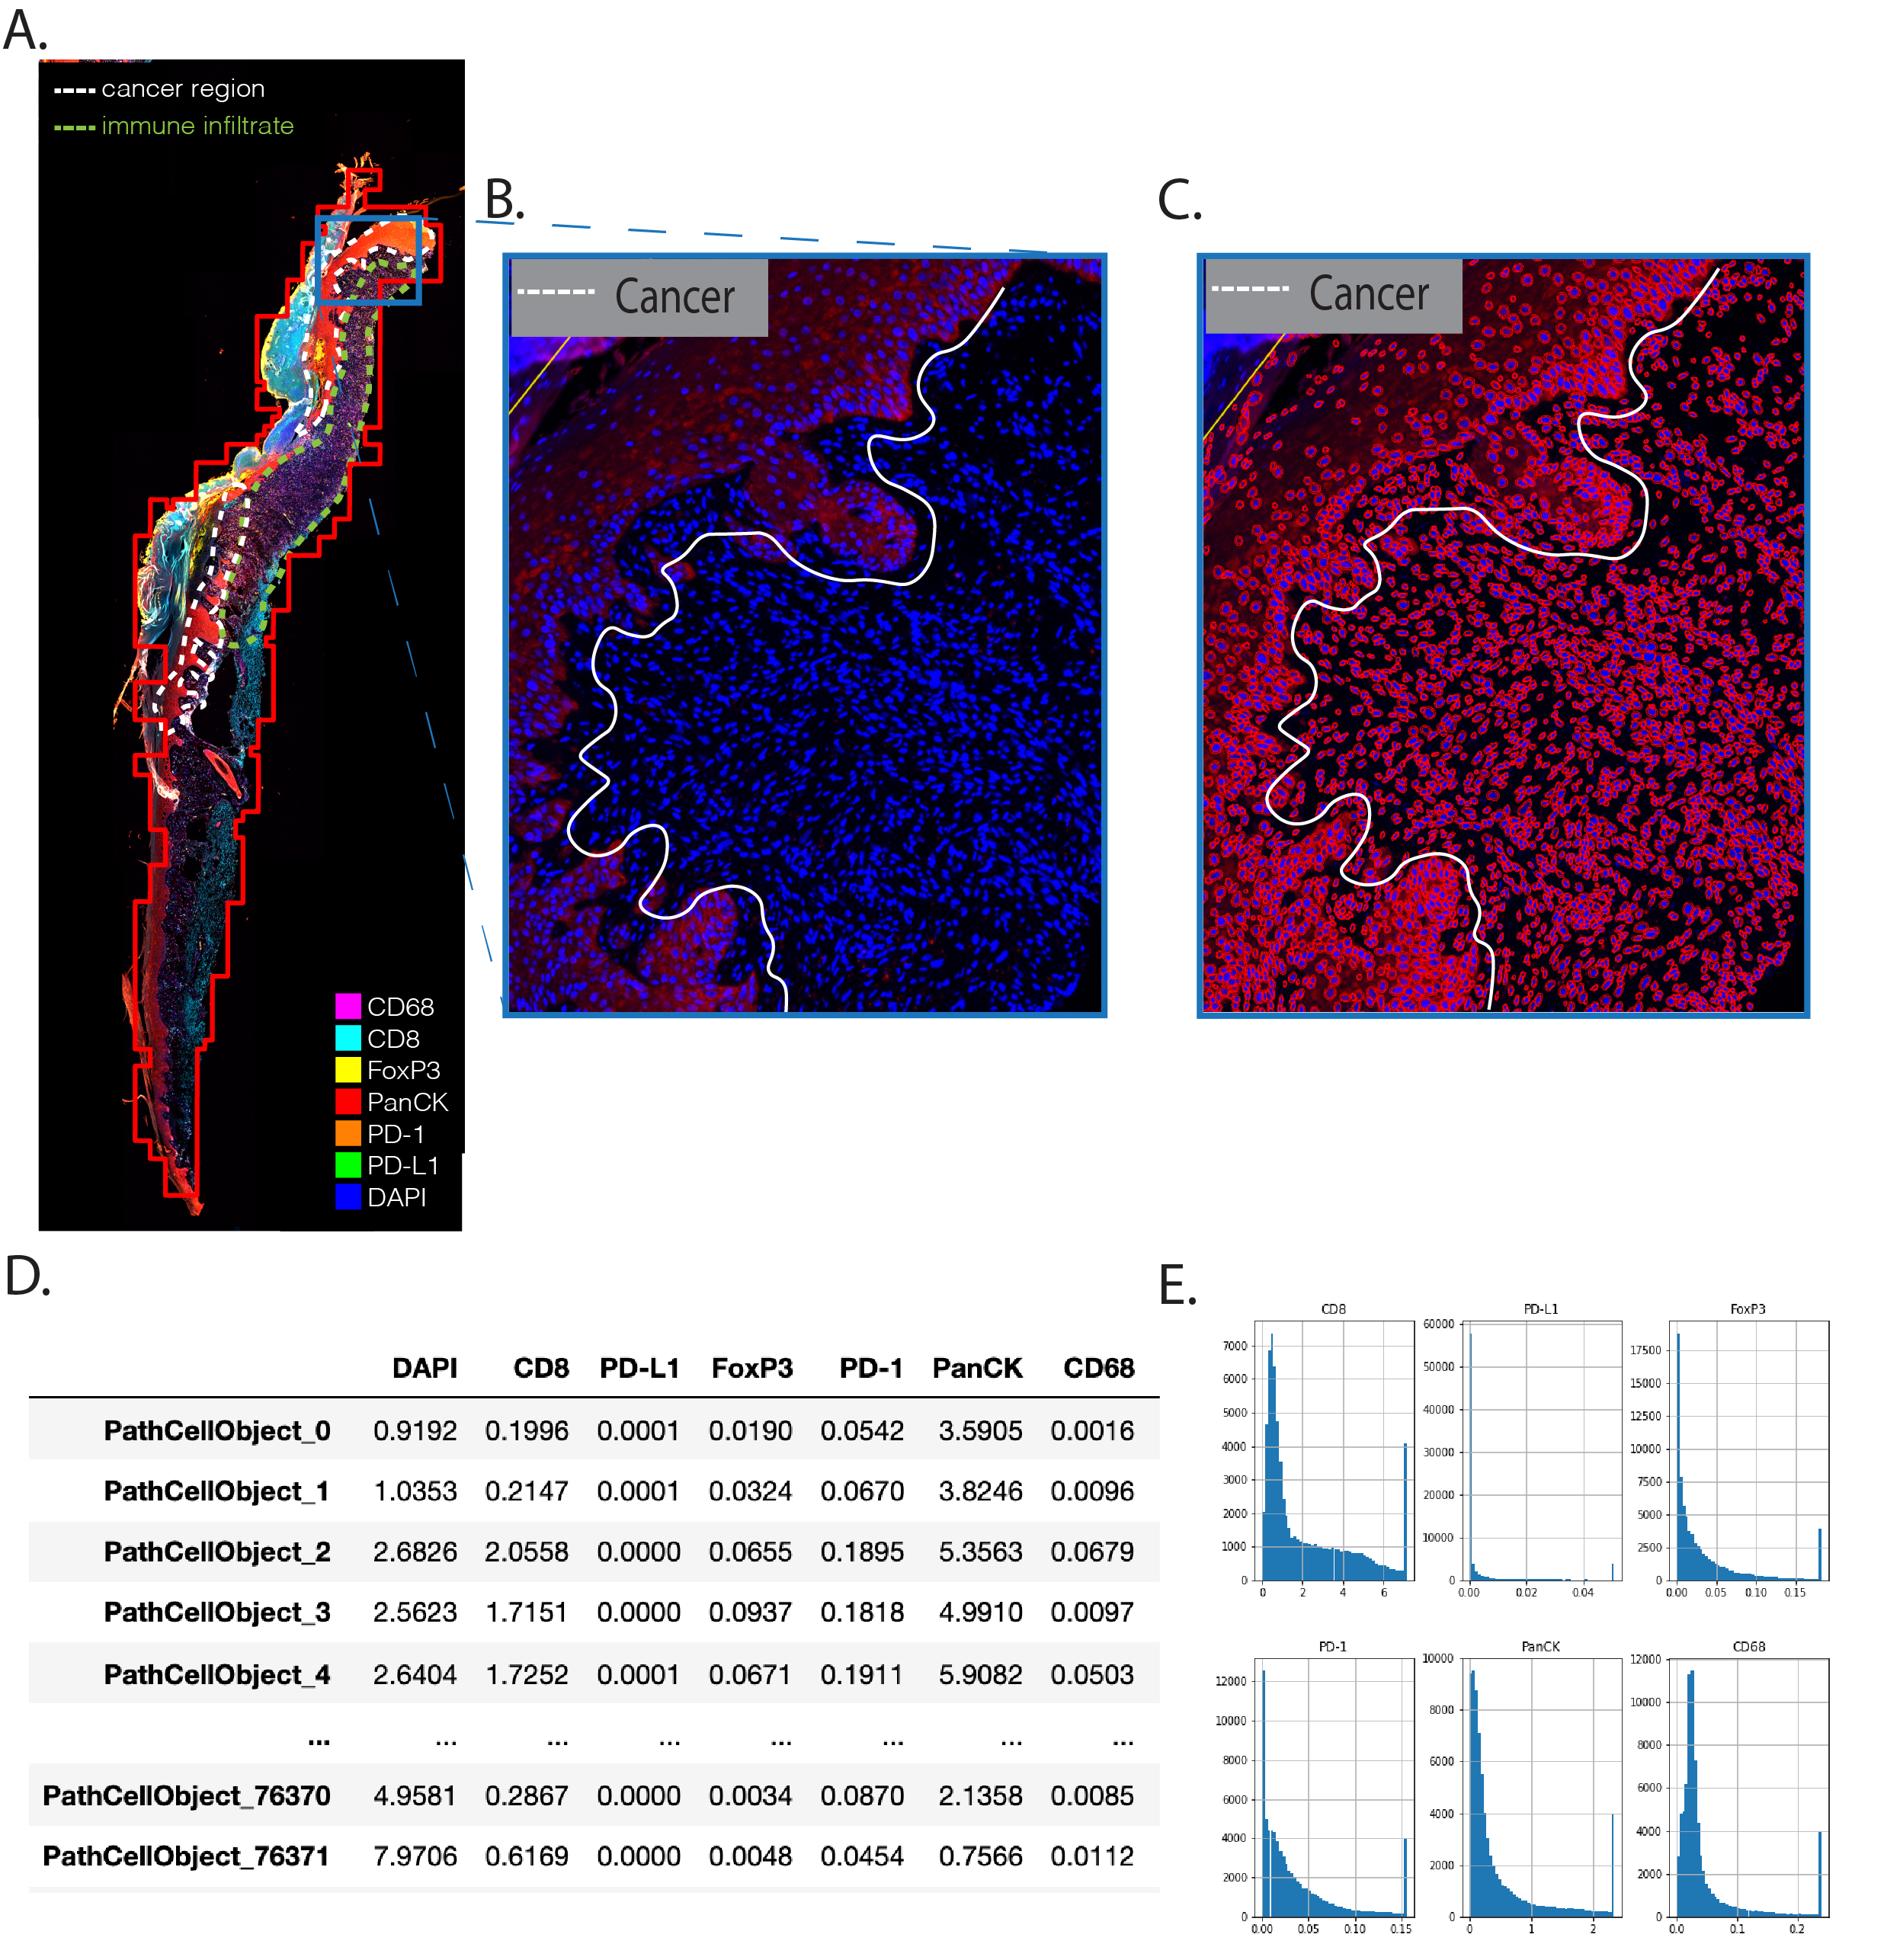
\includegraphics[width=\columnwidth]{Chapter3/Figures/Chap3_Figure1_1.png}
    \caption[Schematic of spatial data preprocessing for cell type annotation.]{ Opal Polaris spatial data preprocessing for cell type annotation. (A) Polaris spatial proteomic data from the SCC patient B18 with the pathological annotation based on tissue morphology. (B) A zoomed-in image of cell the nuclei representation in the DAPI channel (dark blue) and cytokeratin marker expression (PanCK in red) for epithelial cell marker. The annotation line in white colour separates the cancer lesions of the skin from the lower layer. (C) Detection and segmentation of cells from the image using the nuclei channel. (D) The conversion of imaging-based data to single-cell-based data by mapping the  signal for each cell within the cell boundary. (E) Histograms of the expression level of each protein in the panels across all the detected cells}
    \label{fig:Polaris_skin_cancer_preprocessing}
\end{figure}

The cell segmentation process is a crucial step in extracting meaningful information from most multiplexed imaging data, including multiplexed Polaris. For the skin cancer Polaris project, each skin cancer sample contained around $40000\sim 79000$ cells per tissue, depending on the size of the whole slide tissue section. To employ the currently established cell clustering and annotation, the multiplexed Polaris image was transformed into non-imaging-based data through the cell segmentation process (Figure: \ref{fig:Polaris_skin_cancer_preprocessing}A-B) \cite{hickey2021strategies}. We utilized a deep learning model called StarDist \cite{schmidt2018cell} to segment every nucleus in the DAPI channel into individual cell objects across the whole tissue (Figure: \ref{fig:Polaris_skin_cancer_preprocessing}A-B) \cite{hickey2021strategies}. Post segmentation, the protein signal intensity for each cell was normalized to the mean DAPI intensity within the cell boundary, and this value was assigned to the expression level of the corresponding protein (Figure: \ref{fig:Polaris_skin_cancer_preprocessing}B-D). To remove the noisy high background from fluorescent intensities (outliers), we added a custom threshold of $95^{th}$ percentile, which was used to cap the maximum value of each marker (Figure: \ref{fig:Polaris_skin_cancer_preprocessing}D-E). 

After preprocessing and quality check of raw imaging data, the single-cell protein expression data were subsequently scaled and clustered using the Leiden clustering algorithm using scanpy package\cite{wolf2018scanpy}. The result clusters were assessed to determine cell type identity. Using differential expression analysis of each cluster, we were able to identify six major cell types, including epithelial (PanCK+), inmate immune (CD68+), and adaptive immune (CD8+, FoxP3+) cells from all tissue samples. Cells showing very low expression of all six protein markers were classified as "unidentified" and removed from downstream analysis. The spatial coordinate of each cell was retained to facilitate further the construction of the neighbourhood network and spatial analysis of cell-type colocalisation/interaction. 

\subsubsection{Cell segmentation and identification from Imaging Mass Cytometry data}
For our IMC dataset in COAD, the raw data from the imaging system were converted into multichannel images, which later underwent data preprocessing and cell segmentation. During imaging of the IMC platform, a laser is used to ablate and vaporise the tissue pixel by pixel, and the metal probes released from each spot are quantified with a grid of mass spectrometers. Although the IMC platform is also highly multiplexed and powerful, the imaging process produces lower-resolution images compared to multiplexed IF staining (\ie multiplexed Polaris). While every pixel in the Polaris image captures $0.49 \mu m$ in the real tissue, the specification in IMC is $1$ pixel representing $1\mu m$. The IMC image generated discrete ion count signals (counts of heavy metal molecules from labelled antibodies) in contrast to the continuous fluorescence intensity from IHC/IF. The IMC data requires a specialised cell segmentation method. Currently, the IMC image conversion and preprocessing pipeline are being adapted from a pipeline by Bodenmiller Group, one of the founders of the technology (\href{https://github.com/BodenmillerGroup/ImcSegmentationPipeline/blob/development/scripts/imc_preprocessing.ipynb}{IMC preprocessing pipeline}. 

Briefly, the raw IMC data (.mcd file) is converted into a standard image format with multiple channels (Open Microscopy Environment (OME) tiffs), where each channel represents the expression of a protein staining marker (Figure \ref{Chap3:fig:IMC_data_preprocessing}A). Because the signal intensity in IMC has a lower resolution yet is noisier than in Polaris, we manually built a segmentation model to assign pixels to either cell nuclei, cytoplasm, or background. In collaboration with a team member, we assigned the pixel annotation to a subset of cells in the whole ROI using CellProfiler, and Ilastik \cite{carpenter2006cellprofiler, berg2019ilastik}. The trained pixel classification model from Ilastik was performed across the whole dataset to segment the cells from the background (Figure \ref{Chap3:fig:IMC_data_preprocessing}B-D). Since IMC imaging data was generated only for selected ROIs, the number of cells in this project is significantly lower than that in the skin cancer project, ranging from $200$ to $1600$ cells per ROI (approximately 2-3 ROIs per sample). After the cell segmentation, customised single-cell data preprocessing is applied to map signals to a list of cell objects. The mapped single-cell level data was also clipped to remove outliers. Additionally, cells that were either too small (due to  signal noise) or too large (possibly overlapped cells) were filtered from the downstream analysis (Fig: \ref{Chap3:fig:IMC_cell_type_annotation}A-B). By applying the harmony algorithm to single-cell data from 170 ROIS of 52 patients a total of $903,125$ cells were merged for further analysis \cite{korsunsky2019fast}. 

For cell type annotation, differential expression analysis of protein expression across cells identified $10$ major structural cells with high confidence. The first group of cells contained cancer-associated types such as Epithelial/Cancer (E-cadherin and Keratin), proliferative tumour (KI67+), and stromal (Collagen, SM-actin). In the second group of cells, we were also able to annotate key immune cells like B-cells, cytotoxic T-cells, lymphocytes, Natural Killer cells (NK-cells), and macrophages (Fig:\ref{Chap3:fig:IMC_cell_type_annotation}C). For validation, we compared the IMC-identified cell types against pathological annotation. We could align the IMC image to the adjacent section of the H\&E image, which the pathologist annotated with some cell types (Fig:\ref{Chap3:fig:IMC_cell_type_annotation}D). Since our computational results matched well with manual annotation, this gave us confidence in our cell segmentation and clustering approaches before proceeding to the CCC analyses.

\begin{figure}[htp]
    \centering
    \includegraphics[width=0.8\columnwidth]{Chapter3/Figures/imc_histocat_pipeline_v2.png}
    \caption[Illustration of IMC data preprocessing.]{ Summary of the current IMC data preprocessing. (A) From the original IMC of the imaging platform, multi-layer tiff images for the cell segmentation pipeline or single-layer tiff for protein marker visualization. (B) Illustration of the cell segmentation process with two steps. The first step involves manual pattern recognition to create the pixel classification mask with Ilastik \cite{berg2019ilastik}. After pixel classification, the pixel probability map is fed through CellProfiler to generate the mask for each cell in the IMC image. (C) IMC image is highly multiplexing data with each protein signal in an individual tiff image. Therefore we utilise the single-layer tiff image to represent the count/means value of the protein expression in a cell. (D) After the cell segmentation, the protein expression of each cell is measured by projecting each protein channel from the input image to the cell mask.  }
    \label{Chap3:fig:IMC_data_preprocessing}
\end{figure}

\begin{figure}[htp]
    \centering
    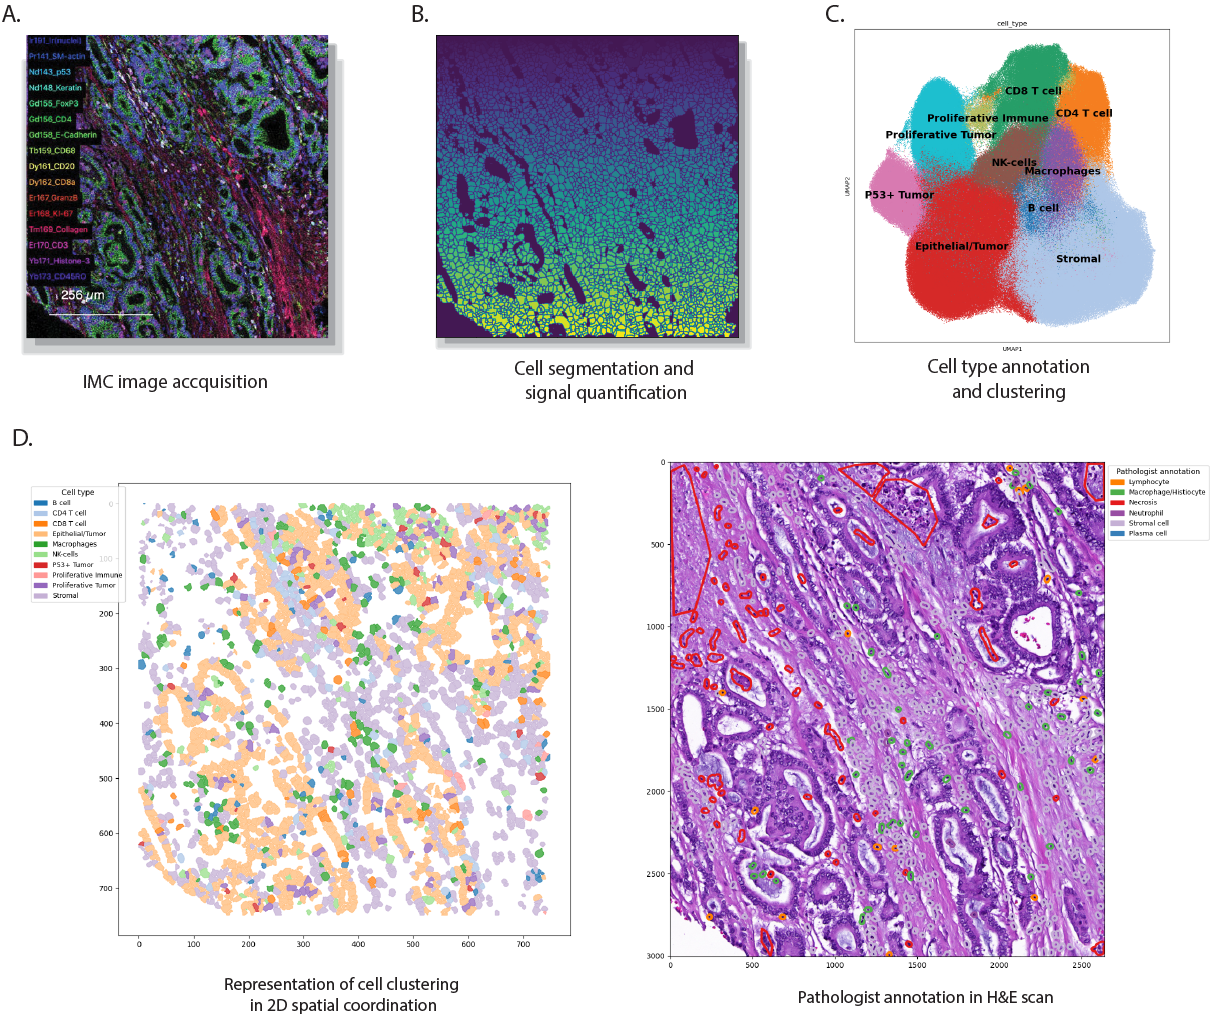
\includegraphics[width=\columnwidth]{Chapter3/Figures/Chapter3_Figure2_IMC_cellID_ver2.png}
    \caption[Cell identification from Hyperion Imaging Mass Cytometry data]{The workflow for the transformation IMC data from multiplexed imaging data to single-cell proteomic matrix (A) A standard mcd file from Hyperion IMC platform was converted into a multiple channel OME-tiff file. Each channel of a tiff image represents a protein staining channel. (B) A pixel classification training dataset was manually generated, and the trained model was  specifically applied to the whole dataset to perform cell segmentation. (C) Cells from multiple ROIs were merged, clustered, and annotated. (D) Annotated cells were plotted back to the original spatial context for validation using pathologist annotations.}
    \label{Chap3:fig:IMC_cell_type_annotation}
\end{figure}
\subsection{Spatial cellular network analyses to detect cell communities}
\label{Chap:3:Community_detection_Method}
Both cell types and the TMEs are important attributes when evaluating the state and heterogeneity of cancer at the tissue level. TMEs can segregate the tissue into multiple cell compartments such as cancer nest, stromal and normal regions. The segregation occurs because different cell types often reside in the same spatial neighbourhood, and the non-random colocalisation of two cell types reflects potential cellular communications. The community detection approach was employed to capture the pattern of spatial features in a cancer tumour. This analysis aims to identify groups or communities of cells that exhibit strong interactions or colocalisation within the tissue. By detecting these communities, we can gain insights into cells' organization and cell distribution patterns within the tumour microenvironment. 

I utilised the K nearest neighbour method to construct the cellular neighbourhood network. In this approach, each cell in the tissue is considered a point process in the Cartesian coordinate system and is connected to its K nearest neighbouring cells in adjacent proximity. This network provided information about the spatial relationships between cells. After constructing the neighbourhood network, I performed the clustering to group the cells from the same neighbourhood with similar local features into the same community. This analysis was applied to all three spatial-proteomic datasets in this chapter to identify the communities of cells within each tissue sample. Additionally, the projection of cell community onto the tissue landscape helps elucidate how cells can perform communication and provide the landscape of cell distribution throughout different tissue sites. 

\subsubsection{Detecting cell communities in skin cancer using spatial network}
\label{Sec:3_cell_communities_and_coocurrence}	%CREATE YOUR OWN LABEL.
Using the cell type clustering information, we sought to identify the regions where cancer and immune cells were highly co-localised and possibly interacted. First, we investigated cell type co-localisation through spatial clustering analysis \cite{schurch2020coordinated}. The spatial features of a cell were extracted by scanning $K$ nearest neighbouring cells surrounding the query cells. The nearest neighbour metric was defined by the Euclidean distance between the cells' $X$ and $Y$ coordinates in the two-dimensional tissue section. For each cell across the tissue, we identified the neighbouring cells using $10$ nearest neighbours within a radius of $100\mu$m from the query cell. Every cell's neighbouring profiles across the tissue were aggregated and clustered using mini-batch K-means clustering. The mini-batch K-means clustering applies the  K-means algorithm on multiple batches of samples, reducing the computational cost of finding the clusters from the large dataset \cite{sculley2010web}. By clustering the cells based on cell neighbourhood profile (\ie spatial features), we can group the cells with the common colocalisation profiles into communities of cells. Additionally, we quantitatively measured the cell composition for each spatial community to identify the cell types enriched for each community. 

We employed cell-type co-occurrence analysis to quantitatively measure the changes in cell localisation through different distance radii. The co-occurrence analysis was inspired by an approach introduced by Tosti et al. \cite{tosti2021single}, first applied for spatial transcriptomics data of human pancreas \cite{tosti2021single}. Briefly, Ripley's K-function was used to summarise the co-occurrence of specific cell types with all other cell types across increasing distance intervals. Therefore, the Ripley K-function calculates the expected number of neighbouring points and compares them with the co-occurrence of random points to determine whether is expected co-occurrence points are clustered, dispersed, or distributed at random patterns. The co-occurrence score can be estimated by the Equation \ref{Eq:Cooc_equation}, which is defined by the fraction of the probability of observing a test cell type $exp$ at the presence of a reference cell type $cond$ ($P_{r}(exp|cond)$) over the probability of observing that test cell type $exp$ $P_{r}(exp)$ at the presence of any other cell type within the same distant interval $r$. At a specific distance, $r$, $Co_{r}$ indicates how high/low $exp$ and $cond$ cell types co-localised compared to random cell types. The co-occurrence scoring is widely used in various fields, including ecology and geography, and has been applied to spatial analysis of proteomic data as a metric of co-localisation in squidpy \cite{palla2022squidpy}. 

\begin{align}
\label{Eq:Cooc_equation}
Co_{r} = \frac{P_{r}(exp|cond)}{P_{r}(exp)} 
% K(t) =  \sum_{i=1}^{n}\sum_{n}^{j}1\{d_{ij} < r\} \\ 
\end{align}

% \subsection{Applying nearest neighbourhood approaches to cell-cell interaction}
% ********* Enter your text below this line: ********
 The samples were scanned and stitched into large whole-slide images ($>2000 \mu m$ in length) while preserving the original form of the biopsy. We adjusted the function to measure the co-occurrence score using a 50$\mu$m interval with $r$ ranging from 0$\mu$m to 600$\mu$m (\ie 95\% of the pairwise distance between the conditional cell type and others). Because the skin biopsies are wide but narrow, the cell type co-occurrence scores are expected to diverge after converging. The comparison of the co-occurrence scores $Co_{r}$ at an increasing distant radius $r$ shows how the co-localisation of two cell types starts dispersing. By applying the co-occurrence score, we aim to ascertain whether cell communities identified by the previous analysis followed true spatial patterns. The function to calculate the conditional probability of cell type co-occurrence at dynamic distance intervals was implemented from the co-occurrence analysis in the Squidpy package \cite{palla2022squidpy}.

\begin{figure}
    \centering
    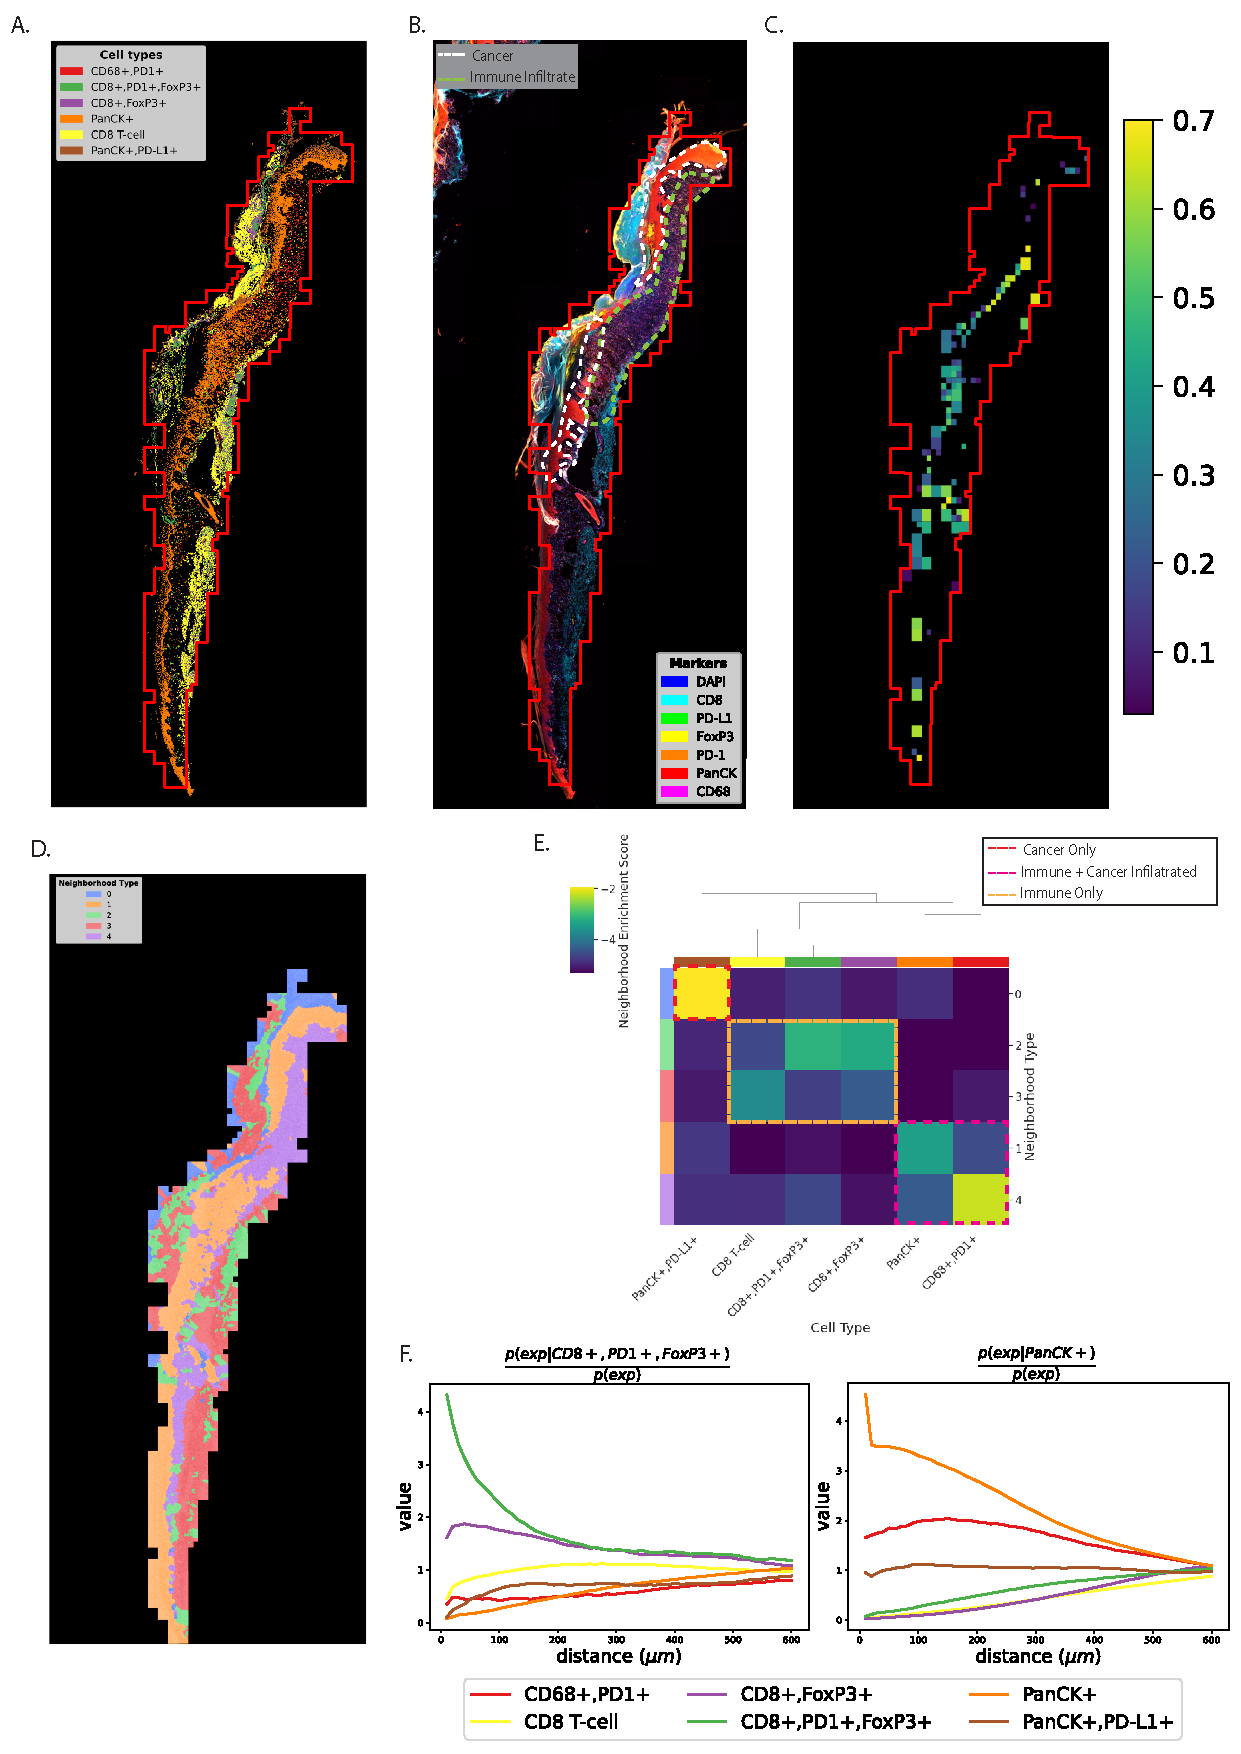
\includegraphics[width=0.8\columnwidth]{Chapter3/Figures/Minh_figure3-01.png}
    \caption[Analyses of Polaris multiplexed imaging of human SCC skin cancer tissue. ]{High-order analyses of Polaris multiplexed imaging data of human SCC skin cancer tissue. (A) Cell type classification through clustering and signal gating of the expression of 6 proteins mapped to single cells. The panel of 6 antibodies was used to profile the protein expression of major interest cell types, including cytokeratin, cancer cells secreting immune inhibitor (PD-L1), and immune cells (CD8 T-cell, NK cells, Macrophages). (B) Pathological annotation of cancer and immune regions, based on tissue morphology. (C) Analysis of co-localisation of the ligand-receptor pairs PD1 and PD-L1, suggesting cancer-immune cell interactions. (D) Voronoi map using the spatial distribution of the cell communities to split the original tissue into multiple regions, representation of distinct cell neighbourhood communities defined via clustering}
    \label{fig:skin_cancer_polaris}
    
\end{figure}

% ***************************************************
\subsection{Extended application to SARS-CoV-2 infection in lung tissues}
Cell type identification from the SARS-CoV-2 dataset was accomplished using starDist, a cell segmentation method \cite{schmidt2018cell}, applied to the multiplex Polaris image. Following cell segmentation, the protein signals were measured within the cell area. To ensure high signal quality and removal of background noise, the threshold of $95^{th}$ percentile was used to filter out mostly noisy signals. Additionally, a quality control step was implemented to exclude cells with too small or too large areas (cell areas less than $5\%$ or more than $95\%$). Subsequently, cells are clustered using the Leiden clustering algorithm \cite{wolf2018scanpy}. Based on the panel of the protein panel, $5$ cell clusters were annotated using the differential expression analysis of cell types, namely NK cells (CD56+), Monocyte/Myeloid (CD15+), Neutrophil (CD66b), cytotoxic T cells (CD8+), and total T cells (CD3+). (Fig. \ref{fig:Chap3_Covid_project}A, B). Among all the clusters detected, those cells with very low expression of all the proteins in the panel were classified as unidentified and excluded from downstream analysis.

Having identified the cell types, the downstream analysis was focused on understanding the immune response in SARS-CoV-2 through spatial analysis of these cells in communities of immune cells. This involved grouping cells into distinct clusters based on their spatial attributes, which are defined by the $10$ nearest neighbouring cells. By clustering cells with similar spatial neighbourhood patterns, we were able to characterize the composition of cell types within each identified community (Fig. \ref{fig:Chap3_Covid_project}C, D). This approach provided valuable insights into the spatial organization and interplay of different cell types within the tissue microenvironment.

\subsubsection{Detecting cell communities and co-occurrence of cell types in colorectal cancer dataset}
Following the cell communities detection approach, we first established the cellular network for all $172$ ROIs from the IMC dataset. Given the lower resolution of the IMC platform ($1\mu m$ is equivalent to 1 pixel in the image), we incorporated an additional distance threshold to define cell neighbourhoods. The neighbouring distance threshold was set to be  $20\mu m$, representing the $97^{th}$ percentile of all distances. The information on neighbouring cell types was aggregated and clustered using mini-batch K-means clustering across the dataset's $903,125$ cells. By applying multiple cluster resolutions, we confidently identified 8 clusters of cell communities. The cell type composition of each community was normalised and scaled, allowing us to annotate the communities where mixed cells colocalised, including B cells, Macrophages and CD4 T cells. Multiple cancer-specific communities were also annotated, including Stromal, bulk tumour, P53+, and proliferative tumour (Fig \ref{fig:colorectal_cancer_IMC}A-C). The community to which the cells were allocated to can be used as a qualitative inspection of the spatial distribution.  

Next, we performed the co-occurrence analysis to the IMC for the colorectal cancer dataset.  We sought to test for the significant co-localization between cancer cell types (\ie Epithelial and Stromal) and immune cell types (\ie CD8 T cell, B cell and CD4 T cell) across ROIs. However, the current co-occurrence analysis could only provide insights into how different cell types form cell communities, and the analysis is limited to a single ROI at a time. Therefore, we leveraged the co-occurrence analysis from section \ref{Sec:3_cell_communities_and_coocurrence} by introducing an additional analysis where we grouped co-occurrence scores of multiple ROIs together and performed the Wilcoxon test to identify the most significant pair of cell types co-occurrence. Specifically, the co-occurrence scores from each ROI were aggregated by the unique $P(exp|cond)-P(exp)$ and formed a distribution of $Co$ across $172$ ROIs. Next, we tested the distribution of $Co$, a pair of expected-conditional cell types, against all remaining pairs. The P-value derived from the test could indicate how the distribution of the co-occurrence scores varied across the $172$ ROIs.
\subsection{Cellular interaction analysis through contact-based approach}
% histocat approach which uses the cell outline
This approach was explicitly applied to the COAD project, using the cell mask from cell segmentation as a reference to construct a cell neighbourhood matrix for each region of interest (ROI). The aim was to identify significantly enriched interactions between or within cell types in the immediate neighbourhood. Firstly, pairwise interactions of every cell were defined by considering the overlapped cell membrane. Using the extended cell segmentation masks (user-defined threshold), the neighbour interaction is defined as if a pair of cells overlap in extended cell boundaries. Two variables were defined, $observing\_celltype$ and $expecting\_celltype$, representing the two cell types in contact. The pairwise interactions were aggregated by the unique connection of cell types of $observing\_celltype$ and $expecting\_celltype$. For each unique pair of $observing\_celltype$ and $expecting\_celltype$, the frequency of interaction was scored by normalising the total interaction count to the total number of $observing\_celltype$. Random permutations were performed by shuffling the cell types of $expecting\_celltype$. For each permutation, the mean of unique pairwise interaction frequency was calculated again. While the interaction between each pair of cells is bi-direction, the pairwise interaction favours one direction connection originated from $observing\_celltype$. Therefore, the pairwise interaction of random permutation was compared to a baseline distribution using two individual one-tail permutation tests within the same image (each ROI). The $P-values$ indicate how significant a pairwise interaction was observed compared to random distribution. The test eventually suggests an interaction or an avoidance between $observing\_celltype$ and $expecting\_celltype$ compared to random observation.

\begin{equation}
\begin{split}
P_{lt} = \frac{ \sum(mean(permutation) \leq mean(real\_data) )}{number\_perm + 1} \\
P_{gt} = \frac{\sum(mean(permutation) \geq mean(real\_data) )}{number\_perm + 1}
\label{chap1:eq:02}
\end{split}
\end{equation}
Where $P_{gt}$ and $P_{lt}$ defined $P$ value for each tail.

Comparing baseline interaction and randomised interaction of every individual image can identify the differences in frequency (probability) of the connectivity between specific cell types in that tissue compared to the background. By using the extended cell mask boundary, the randomisation of two neighbouring cells in this analysis approach is not directly affected by absolute cell number or the size of the image. Yet the frequencies of cell types present and the relative quantities are essential. The absolute cell number or the image size does not directly affect the neighbourhood analysis; only the frequencies of cell types present and the relative quantities are important. 

\begin{figure}[hp]
    \centering
    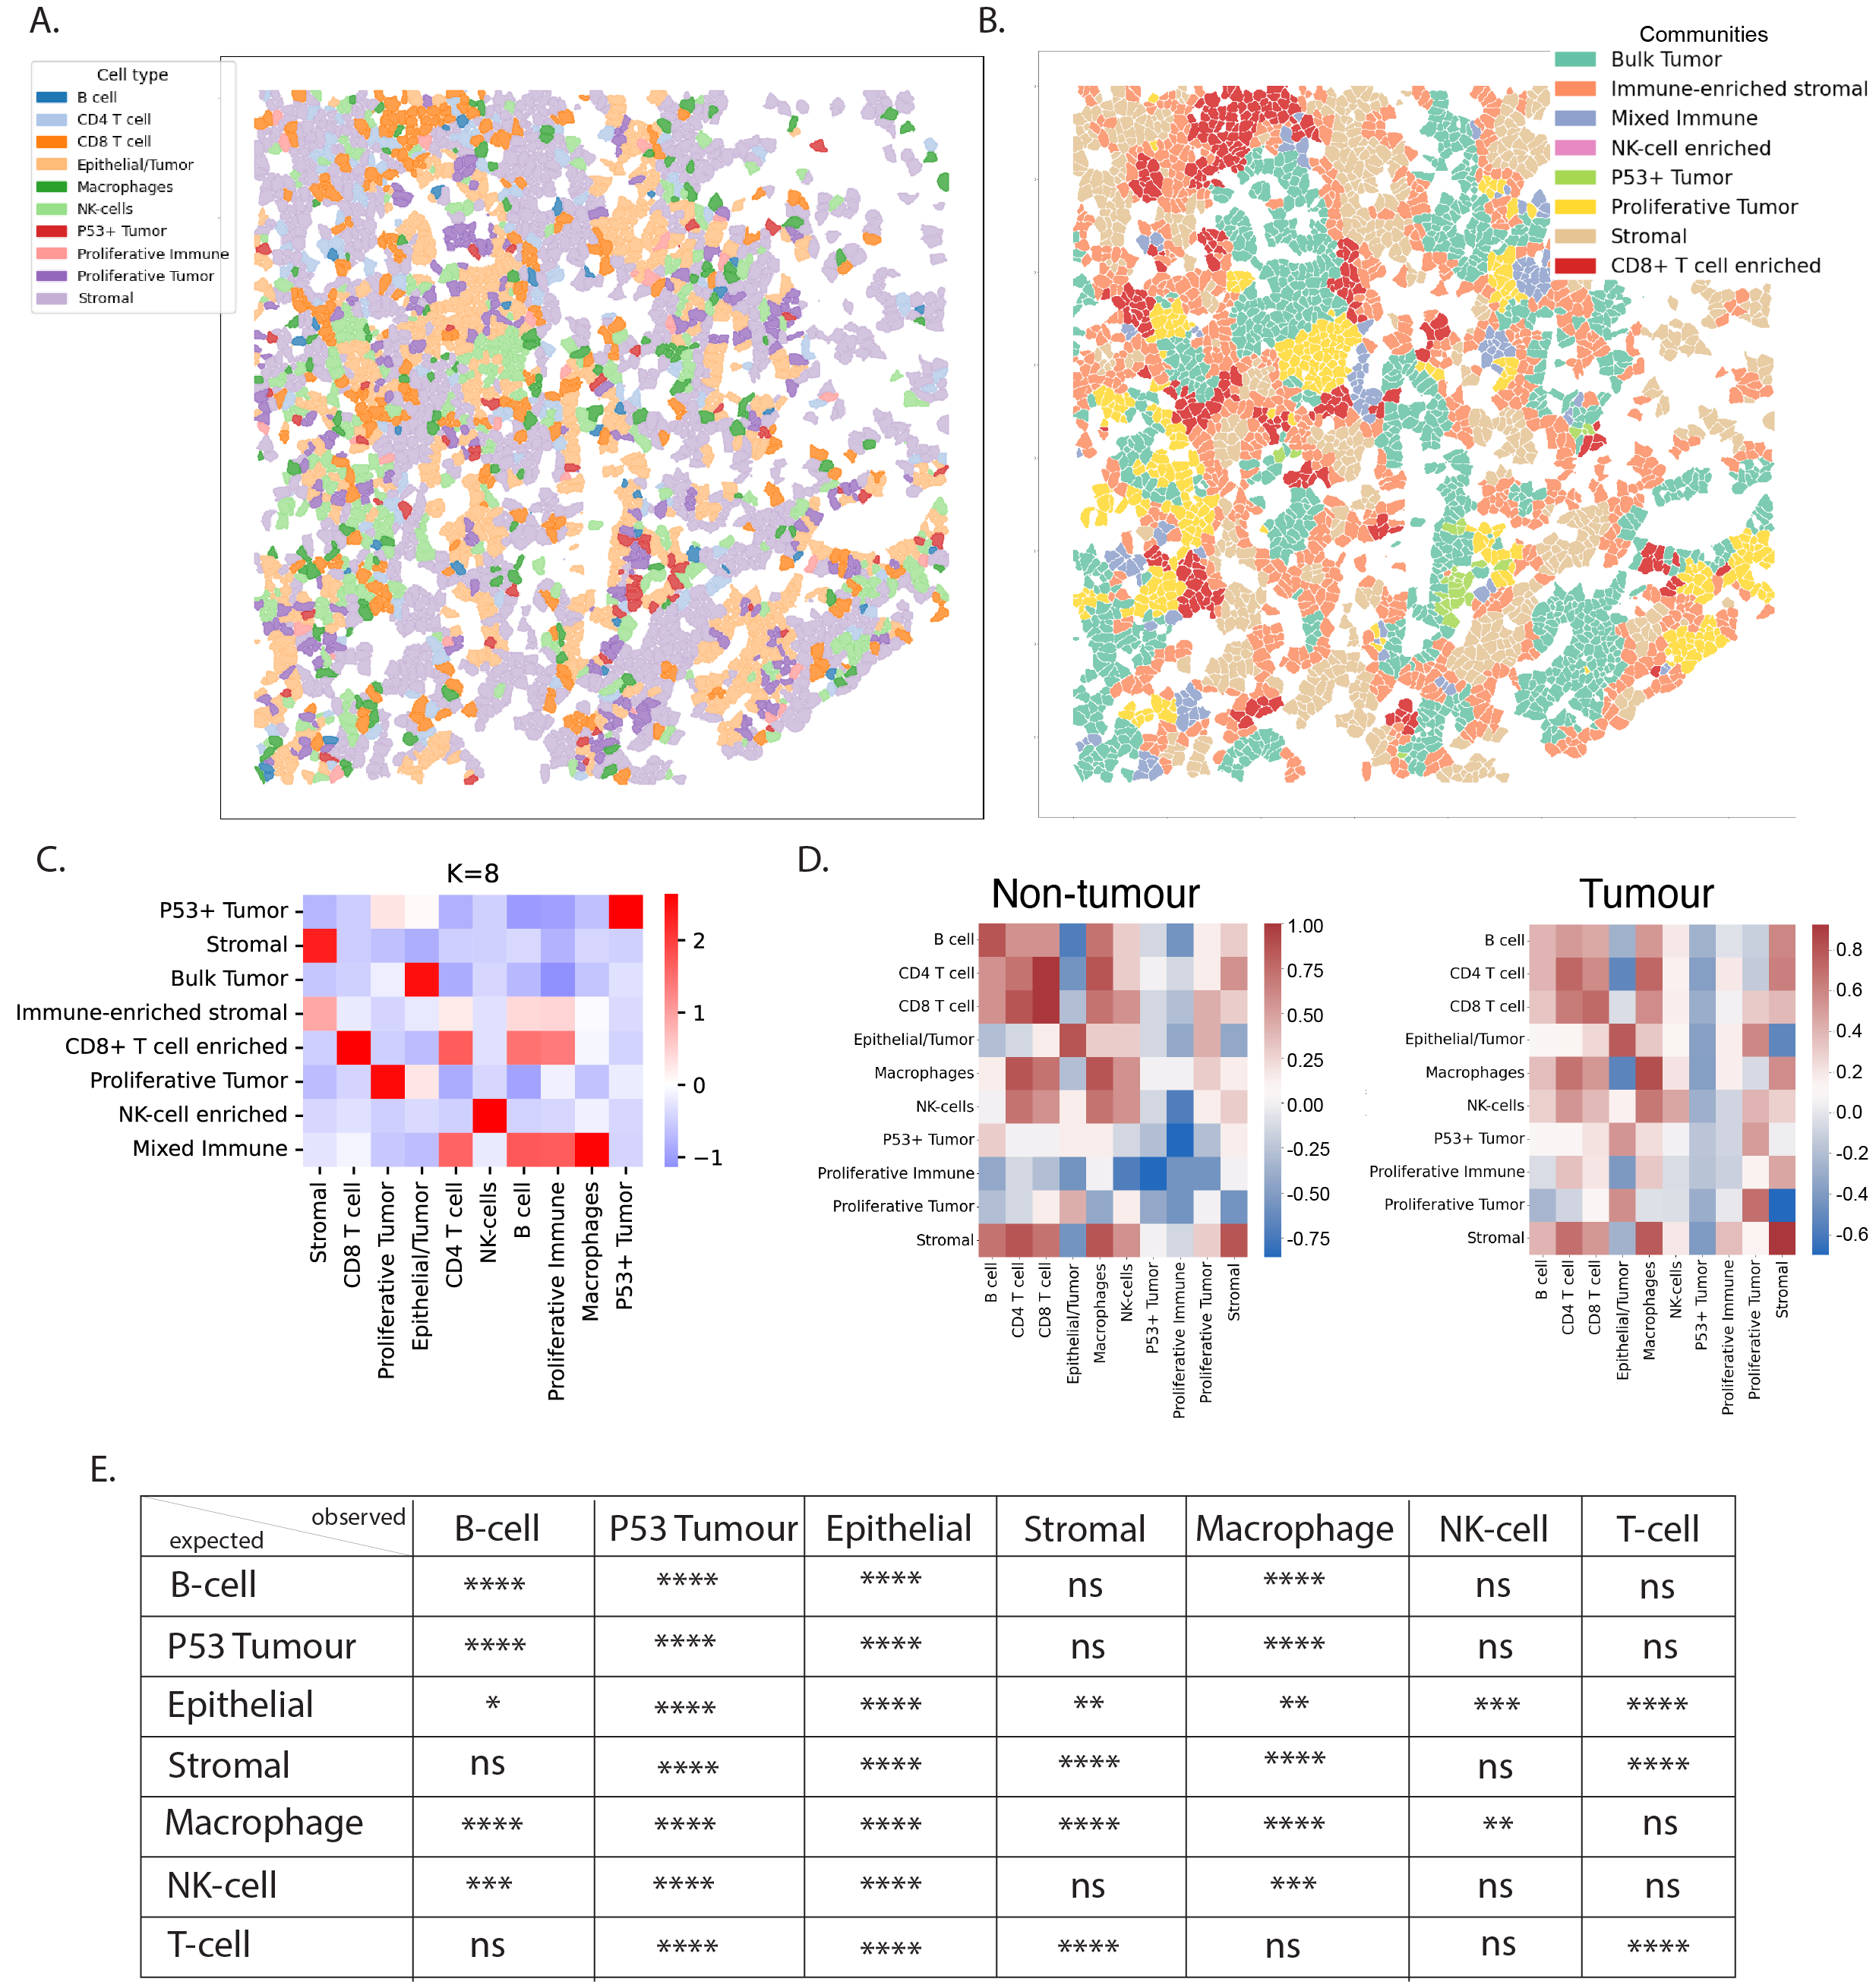
\includegraphics[width=0.94\columnwidth]{Chapter3/Figures/Chap3_figure4_v2.png}
    \caption[High-order cell neighbourhood analysis of IMC data]{High-order cell neighbourhood analysis of IMC data (A, B) The cell type and equivalent cell communities detection results of the ROI from patient ID CR020 (C) Cell type composition of each cell community can inform the function of the community  (D) The pairwise cell-cell interaction through the contact-based approach allows the identification of the interaction or avoidance between each pair of cell types. Grouping the significant interaction/avoidance score between tumour and non-tumour ROIs could inform the association of cell-cell interaction and tissue conditions. (E) A summary of significant co-occurrence scores across all combinations of observed and expected cell types. The number of asterisks indicates the level of significance from low to high.}
    \label{fig:colorectal_cancer_IMC}
    
\end{figure}

\begin{figure}[hp]
\renewcommand{\figurename}{Figure}
    \centering
    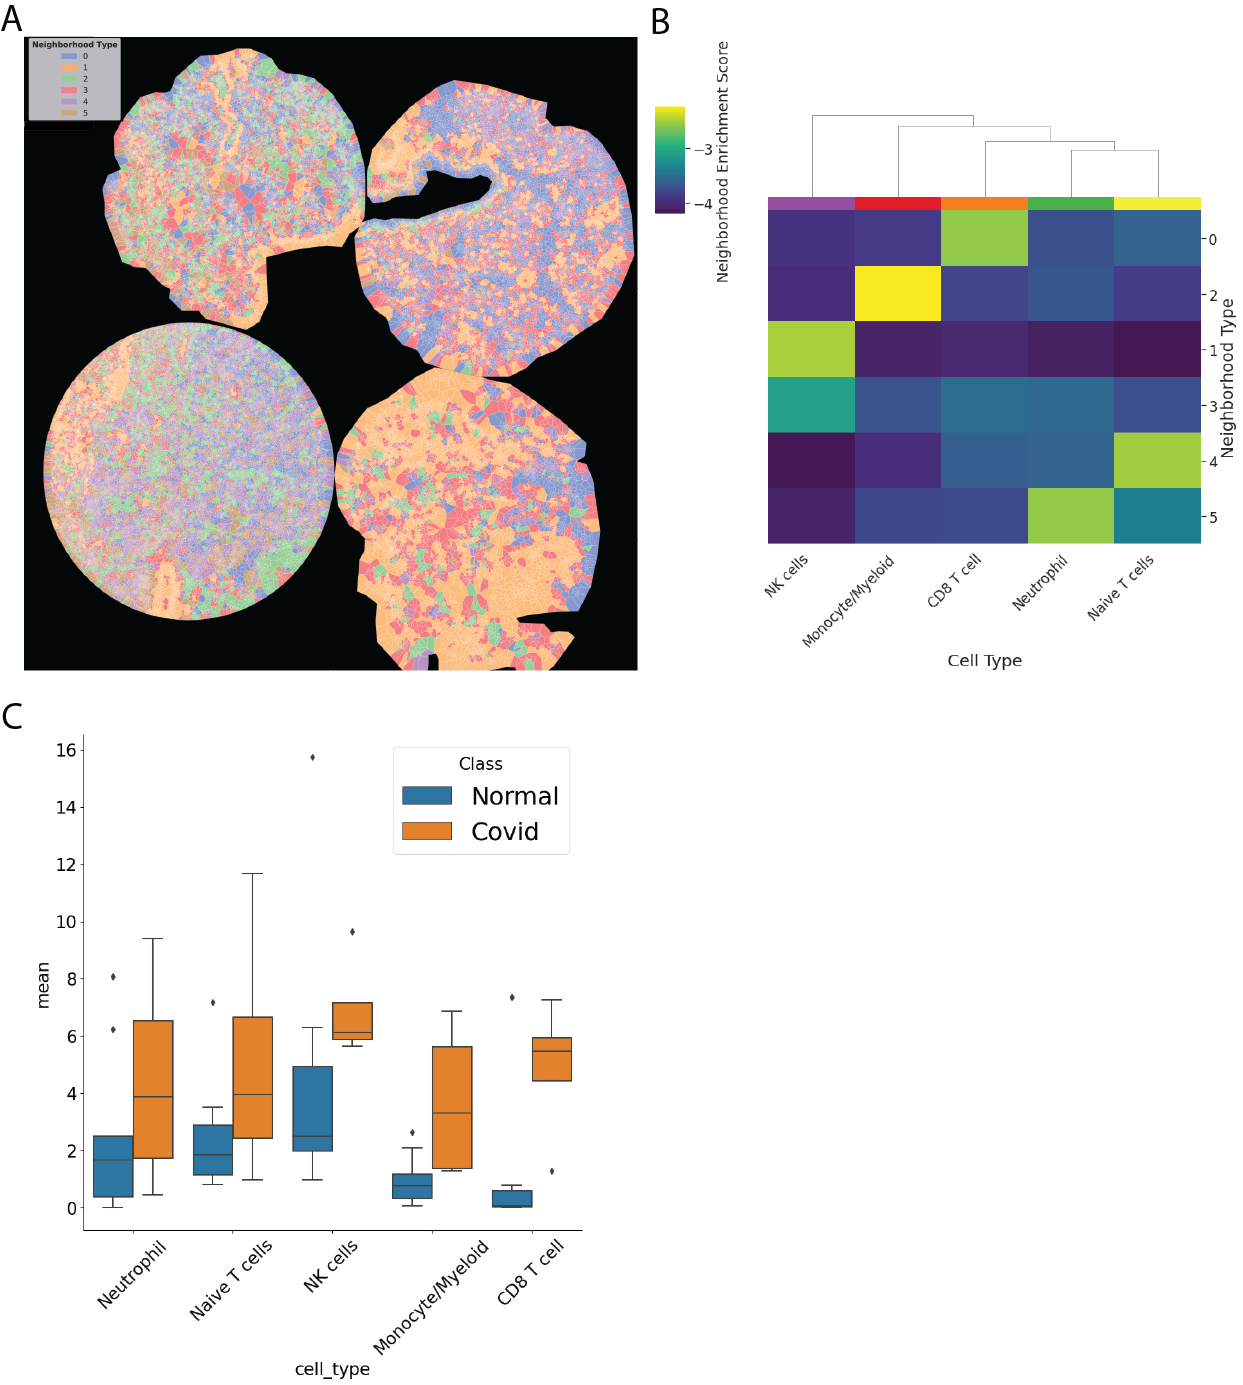
\includegraphics[width=0.9\columnwidth]{Chapter3/Figures/Chap3_Apendix_covid.png}
    \caption[Analysis results in Covid tissue samples using multiplexed Polaris]{Extended analysis results in Covid lung tissue samples using multiplexed Polaris. (A) Multiplexed IHC data of four Covid-infected lung tissue using the multiplexed Polaris imaging platform. (B) Comparison of cell type proportions between COVID-19-infected and uninfected samples. Y-axis shows the mean cell type percentage between replicates (4 COVID-19 and 5 uninfected samples) (C) Voronoi diagram of cell communities detection in Covid samples. (D) Heatmap of cell type decomposition of each cell community detected in (A).}
    \label{fig:Chap3_Covid_project}
\end{figure}

\subsection{Developing STRISH for cell co-localisation testing using spatial proteomic data}
\label{Sec:3.Cell_colocalisation_PD1_PDL1}	%CREATE YOUR OWN LABEL.
After the first version of the STRISH package, some extended features were made to turn the STRISH pipeline into a highly adaptable framework. These additional features allow the STRISH package to effectively handle spatial proteomic data for analysis. We reasoned that the majority of multiplexed imaging technologies that capture gene or protein expression at the subcellular level could be processed using a similar workflow. Collectively, the data preprocessing includes stitching images produced by the Polaris into a multichannel image. Subsequently, cell segmentation and protein expression measurement were applied to extract information from the imaging data into a single-cell protein expression format \cite{shakya2020immune, liu2019comparison, aghaeepour2013critical}. These additional functionalities enable the STRISH package to handle diverse spatial proteomic datasets and facilitate the comprehensive analysis of spatially resolved gene or protein expression patterns.

We further applied the scanning window strategy from the STRISH pipeline to the whole slide tissue to identify the co-localisation of PD-L1 positive T-cells (CD8+) and PD1 positive epithelial cells (PanCK+). The STRISH approach initiates by partitioning the Polaris image into four distinct non-overlapping tiles, each constituting one-fourth of the original slide scan's size. These large tiles are subsequently subdivided into smaller windows iteratively until a predetermined cell count threshold per window is achieved. The windows containing cells expressed target pairs of proteins, PD1 and PD-L1, are then scored to measure the density of cell type within each window. The scores are then normalised across the windows and used to plot a heatmap showing the co-localisation of the two markers. This methodology allows for the thorough finding of the spatial relationship between PD-L1 positive T-cells and PD1 positive epithelial cells across the tissue sample.

\section{Results}
\subsection{Highly multiplexed Polaris data reveal cell communities in skin cancer}
For the Polaris skin cancer dataset, we identified the cell types presented using the panel of 6 antibodies (Table: \ref{table:Chapt3_DataInfor}). Using Leiden clustering and differential expression analysis of the protein expression between cell clusters, we identified $6$ major cell types, including epithelial cells (PanCK+), inmate immune cells (CD68+), and adaptive immune cells (CD8+, FoxP3+) (Fig: \ref{fig:skin_cancer_polaris}A). Among all the clusters detected by the Leiden clustering, those cells with very low expression of all the proteins in the panel were classified as unidentified and removed from downstream analysis. The cell identifications were plotted back to the original spatial context for validation (Fig: \ref{fig:skin_cancer_polaris}B-D).  

Next, we investigated cell type co-localisation more broadly using spatial community analysis. We performed a clustering analysis to group tissue regions with similar local densities/compositions of various cell types, which for patient B18 resulted in the identification of five cell communities distributed across the tissue \ref{fig:skin_cancer_polaris}D). Quantitative assessment of cell composition in each community allowed us to deduce biologically interpretable features of these communities (Fig: \ref{fig:skin_cancer_polaris}D). Notably, communities 2 and 3 consisted of scattered immune cells, while community 1 appeared to have a very high density of epithelial cells positive with PD-L1. The known biological process could explain this and the tissue structure that cancerous epithelial cells tend to reside densely around the cancer nest and the presence of immune cells under the epidermis layer (Fig: \ref{fig:skin_cancer_polaris}B, E).

On the other hand, clusters 1 and 4 contain mixed epithelial and immune cell populations in the same communities. Comparing the distribution of cell communities and tissue annotation (Fig: \ref{fig:skin_cancer_polaris}B) suggested that the clusters 2, 3 and 4 highly aligned with the stromal microenvironment communities (Fig: \ref{fig:skin_cancer_polaris}D). Of note, using our STRISH test (result described in more detail later), we found spatially-specific interactions between PD-1 and PD-L1 along the edge of cancer and immune cell communities (Fig: \ref{fig:skin_cancer_polaris}C).

\subsection{Spatial analysis of Polaris data for cellular profiling interaction via PD1 and PD-L1}
We further sought to detect the local co-localisation of the L-R pair PD-1 and PD-L1, well-known signalling molecules used in immune and cancer cell interaction \cite{pardoll2012blockade} by applying the STRISH package to spatial proteomic data.  We employed the STRISH pipeline to automatically and unbiasedly scan for regions containing T-cells double positive for CD8 and PD-1 in the immediate proximity of cancerous epithelial cells, which themselves are double positive for PanCK and PD-L1 (Fig \ref{fig:skin_cancer_polaris}C). Interestingly, for patient B18, we found that the PD-1+ immune cells and PD-L1+ epithelial cells mostly co-localised at the interface of cancer and immune infiltration, as defined by a pathologist’s annotation (Fig \ref{fig:skin_cancer_polaris}A). Similar patterns were observed by applying the STRISH pipeline to the tissue samples from patients B18 and E15 (Fig: \ref{fig:Chap3_figure3_zoom_in}), and similar results are found in (\ref{fig:Chap3_figure6}). Visual inspection of positive and negative windows (Fig: \ref{fig:Chap3_figure3_zoom_in}A-D) shows the unique new feature of scanning window approach from STRISH in detecting local co-expressing cells of the L-R pairs, in contrast to other methods that only detect the co-expression of two or more proteins from the same cell. 

Quantitative assessment of cell composition in each community allows us to deduce biologically interpretable features of these communities (Fig: \ref{fig:skin_cancer_polaris}D-E). Particularly, community 0 has a very high density of PD-L1+ epithelial cells, while communities 2 and 3 are enriched for three types of CD8+ T cells. Visual inspection of the location of communities 2 and 3 reveals their spatial proximity, which may be explained by the tendency of cancerous epithelial cells to reside densely around the cancer nest, and for immune cells to sit under the epidermis layer \cite{herrscher2020immune}. We also observed that communities 1 and 4 grouped closely together (Fig: \ref{fig:skin_cancer_polaris}E), and these communities contain both cancer and immune cell populations. The spatial distribution of mixed cancer/immune communities (Fig \ref{fig:skin_cancer_polaris}D) aligns with the spatially-specific interaction observed between PD-1 and PD-L1 along the interface between cancer and immune cells (Fig: \ref{fig:skin_cancer_polaris}C).

\begin{figure}[htp]
    \centering
    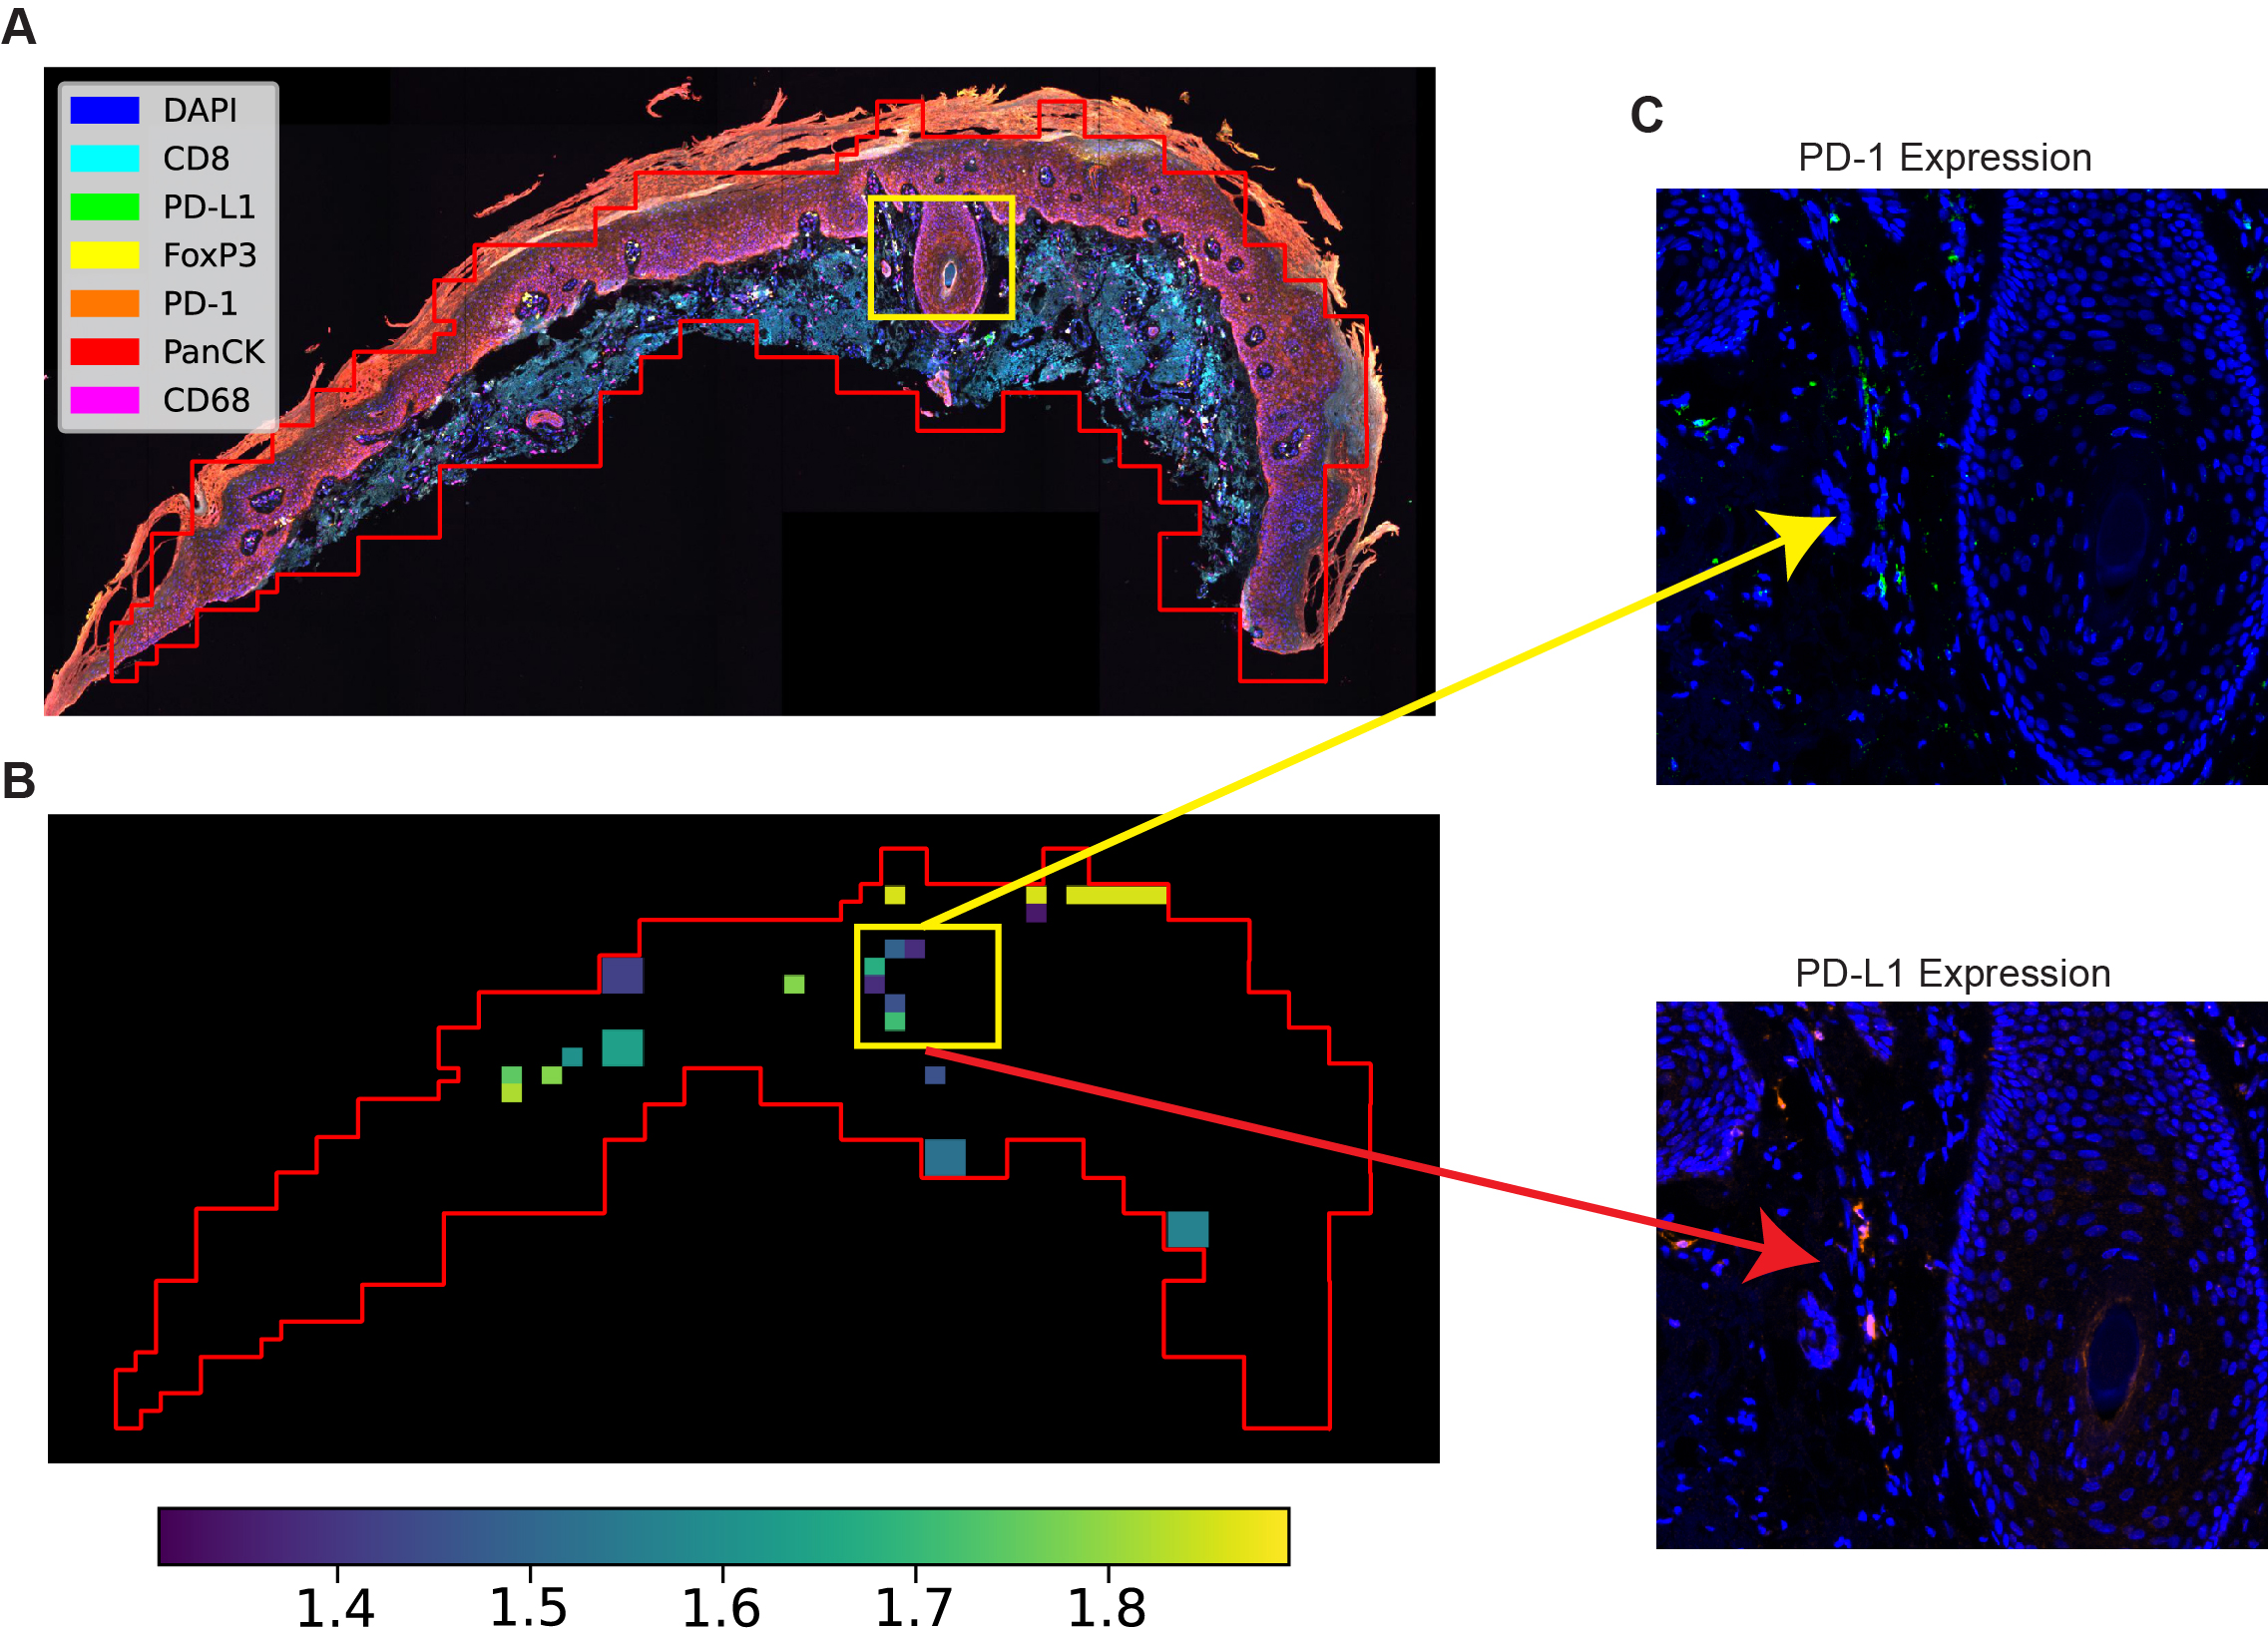
\includegraphics[width=0.8\columnwidth]{Chapter3/Figures/Chapter2_Fig3.jpg}
    \caption[STRISH application to protein data.]{STRISH application to protein data. (A) The multiplexed Polaris image of tissue from the SCC patient (ID E15). (B) STRISH heatmap (activity map) suggesting the tissue locations with high (yellow colour) or low (dark colour) level of protein local co-expression after the statistical test for the ligand-receptor pair PD-1 and PD-L1 (the value shown in the colour bar indicate negative log p-values). The tissue contour was plotted using the windows of neighbouring cells identified by STRISH. (C) A close-up visualization of the areas identified as the existing cell's local co-expression of PD-1 and PD-L1 by STRISH.}
    \label{fig:Chap3_figure3_zoom_in}
\end{figure}

By using the co-occurrence score to summarise the co-localisation of two reference cell types, including CD8 T-cells and epithelial (PanCK+), we investigated the immune-only (communities 2 and 3) and cancer-immune (communities 1 and 4) communities in greater detail. When PD-1+ T cells were set as the reference cell type, these cells were found to co-occur with all three T cell types (\ie with themselves, CD8+ T cells, and FoxP3+ CD8+ T cells) at a significantly higher rate than a random distribution by 2 to 4 times, across a range of distances from $0\mu m$ to $400 \mu m$, (Fig: \ref{fig:Polaris_skin_cancer_preprocessing}F). Similarly, PanCK+ was also found to be co-occurred with the CD68+ and PD1+ double-positive clusters, consistent with the result from our community detection analysis (Fig: \ref{fig:Polaris_skin_cancer_preprocessing}A, F).    

\subsection{Identification of immune cell types and communities of cells in SARS-CoV-2 infected lung}
To understand changes in the spatial organisation of cells in lung tissue sections infected by SARS-CoV-2 at cell type levels, we applied the multiplex Polaris imaging to lung tissues (4 Covid infected and 5 control samples). Through cell segmentation and computational clustering of cell type, we identified five immune cell populations from the image data,  including NK cells, Monocyte/Myeloid, Neutrophil, cytotoxic T cells, and total T cells (Fig. \ref{fig:Chap3_Covid_project}A, B). The comparison of cell type proportion between SARS-CoV-2 infected and control samples showed a higher density of immune cells in the infected samples. Significantly, we observed an increase in NK cells, Myeloid and cytotoxic T cell (CD8 T cells) populations in COVID-19-infected samples compared to uninfected samples (Fig \ref{fig:Chap3_Covid_project}B). The increase in CD8 T cell and Neutrophil numbers has been previously reported in COVID-19 studies using single-cell data analysis \cite{stephenson2021single}.  

The spatial analysis of cell communities in SARS-CoV-2 infected samples provided insight into the distribution of cells around the airway. Our findings revealed the presence of six distinct communities (Fig \ref{fig:Chap3_Covid_project}C, D), each characterized by unique spatial neighbourhood patterns. Notably, the first three communities (0,1 and 2) were predominantly located around the airway in the infected samples showing enrichment for NK cells, Myeloid and CD8 T cells (Fig \ref{fig:Chap3_Covid_project}C). This finding aligns with the comparison of cell proportion between infected and uninfected samples previously, which further supported the notion of immune responses specific to the SARS-CoV-2 virus \cite{stephenson2021single}. The identification of specific cell types enriched in each community strengthens the evidence for immune cells colocalised to perform immune reactions against the virus. (Fig \ref{fig:Chap3_Covid_project}D). Overall, our analysis demonstrated the versatility of considering spatial attributes in understanding immune reactions to not only cancer cells but also the response to pathogens such as the SARS-CoV-2 virus. 

% \subsection{Identifying cell communities from Hyperion Imaging Mass Cytometry data}
\subsection{Cell community and neighbourhood enrichment analyses in colorectal cancer dataset}
The cell segmentation process allows us to establish the single-cell protein expression matrix of $903,125$ cells from the IMC dataset (Fig: \ref{Chap3:fig:IMC_data_preprocessing}). Next, we applied the Leiden clustering algorithm and differential expression analysis using the IMC panel of 16 antibodies (Table: \ref{table:Chapt3_DataInfor}). By examining the differential expression of molecular protein signatures of each cell cluster, we identified three key cell types that are associated with colorectal cancer, including Epithelial/Cancer (E-cadherin and Keratin), proliferative tumour (upregulated KI67), and stromal (highly expressed Collagen, SM-actin). Additionally, various immune cells were identified, namely, B-cells (CD20+), cytotoxic T-cells (CD8+), lymphocytes (CD4+), Natural Killer cells (FoxP3+), and macrophages (CD68+) (Fig: \ref{Chap3:fig:IMC_cell_type_annotation}C-D, \ref{fig:colorectal_cancer_IMC}A). To validate and refine the cell segmentation, the IMC-based cell type identification was qualitatively compared to the pathologist annotation on the H\&E image, and we found a high level of consistency.  

In addition to identifying individual cell types, we aimed to explore the spatial organisation and composition of local regions within the colorectal cancer tissue microenvironment. Using clustering of cell neighbourhood, we confidently identified $8$ communities of cells representing the $4$ major tumours specific and $4$ immune-enriched microenvironments (Fig: \ref{fig:colorectal_cancer_IMC}B). Notably, among these communities, we observed the formation of two specific communities: P53+ tumours and bulk tumour communities. These communities exhibited a high enrichment of P53+ epithelial cells and Epithelial/Cancer cells, indicating their association with tumours characterized by P53 expression (Fig: \ref{fig:colorectal_cancer_IMC}C). Additionally, we also annotated two communities of cells that displayed the dominant cell types enriched for CD8 T cells and NK cells. These communities provide a high-level interpretation of the spatial distribution and interplay of various cell populations within the colorectal cancer microenvironment.     

The cell community analysis can provide the overall estimation of how a group of cell types colocalised in close proximity. However, the chance of a pair of cell types to be colocalised in a community can vary as the distance between  pair-wise co-occurrences of cell types can ch.  
%We could observe a high enrichment of cancer cells with epithelial cells at the first $200\mu m$ interval. While the co-occurrence analysis could provide insights into how different cell types form cell communities, the analysis is limited to a single ROI at a time. The table embedded in the Figure\ref{fig:colorectal_cancer_IMC}E shows the significant test of occurrence scores between every pair of cell types in our dataset. 
% To improve STRISH, Patients diagnosed with advanced BCC/SCC would be beneficial from the successes of immunotherapy observed in melanoma. 

\section{Discussion}
This chapter showcases the versatility of cell-cell interaction analyses through the applications to two different cancer datasets and the extension to investigating SARS-CoV-2 infections. Using multiplexed spatial proteomic data, I presented multiple spatial analysis approaches to identify cell communities and cellular communication in skin cancer and colorectal cancer. As the spatial proteomic platforms perform tissue imaging differently, we addressed some limitations of converting the imaging data to single-cell data and introduced quality control steps for data preprocessing. Cross-validation through combining multiple spatial analyses was demonstrated as a powerful tool for deducing significant interactions in a biological tissue context.   

Notably, the extension of STRISH application to multiplex Polaris data suggests the very broad applicability of this analysis pipeline to the vast amount of protein fluorescence imaging data. The package particularly focuses on cell-cell interaction analyses with applications to spatial transcriptomic and proteomic data. However, it is essential to note that STRISH should not be employed in isolation but rather in combination with other tools for data normalisation and cell-type clustering. Other spatial analysis packages such as Giotto \cite{dries2021giotto} and squidpy \cite{palla2022squidpy} also provide cell neighbourhood enrichment analysis functions through L-R pairs. Such functions, however, can be used mostly for exploratory analysis. Here, we extended the application of the STRISH package, which can be incorporated into data exploration and validation of cellular interaction through ligand-receptor pairs. 

For the second project using the multiplexed IMC platform on the colorectal cancer samples, spatial analysis and permutation tests were applied to identify the cell types, communities of cells and the possible interaction between different cell types. Combining the multiple ROIs and tissue samples for survival prediction and clinical outcome is another important analysis that I am going to implement and present in Chapter \ref{Chap:4}. The next goal of this thesis is to develop a holistic framework to work with multiple samples and the potential to extend to multimodal spatial-omics data. This allows us to differentiate the characteristics of cell-cell communication and communities throughout cancer tissues across multiple patients. 

% \section{Appendix}
\begin{figure}[htp]
\renewcommand{\figurename}{Figure}
    \centering
    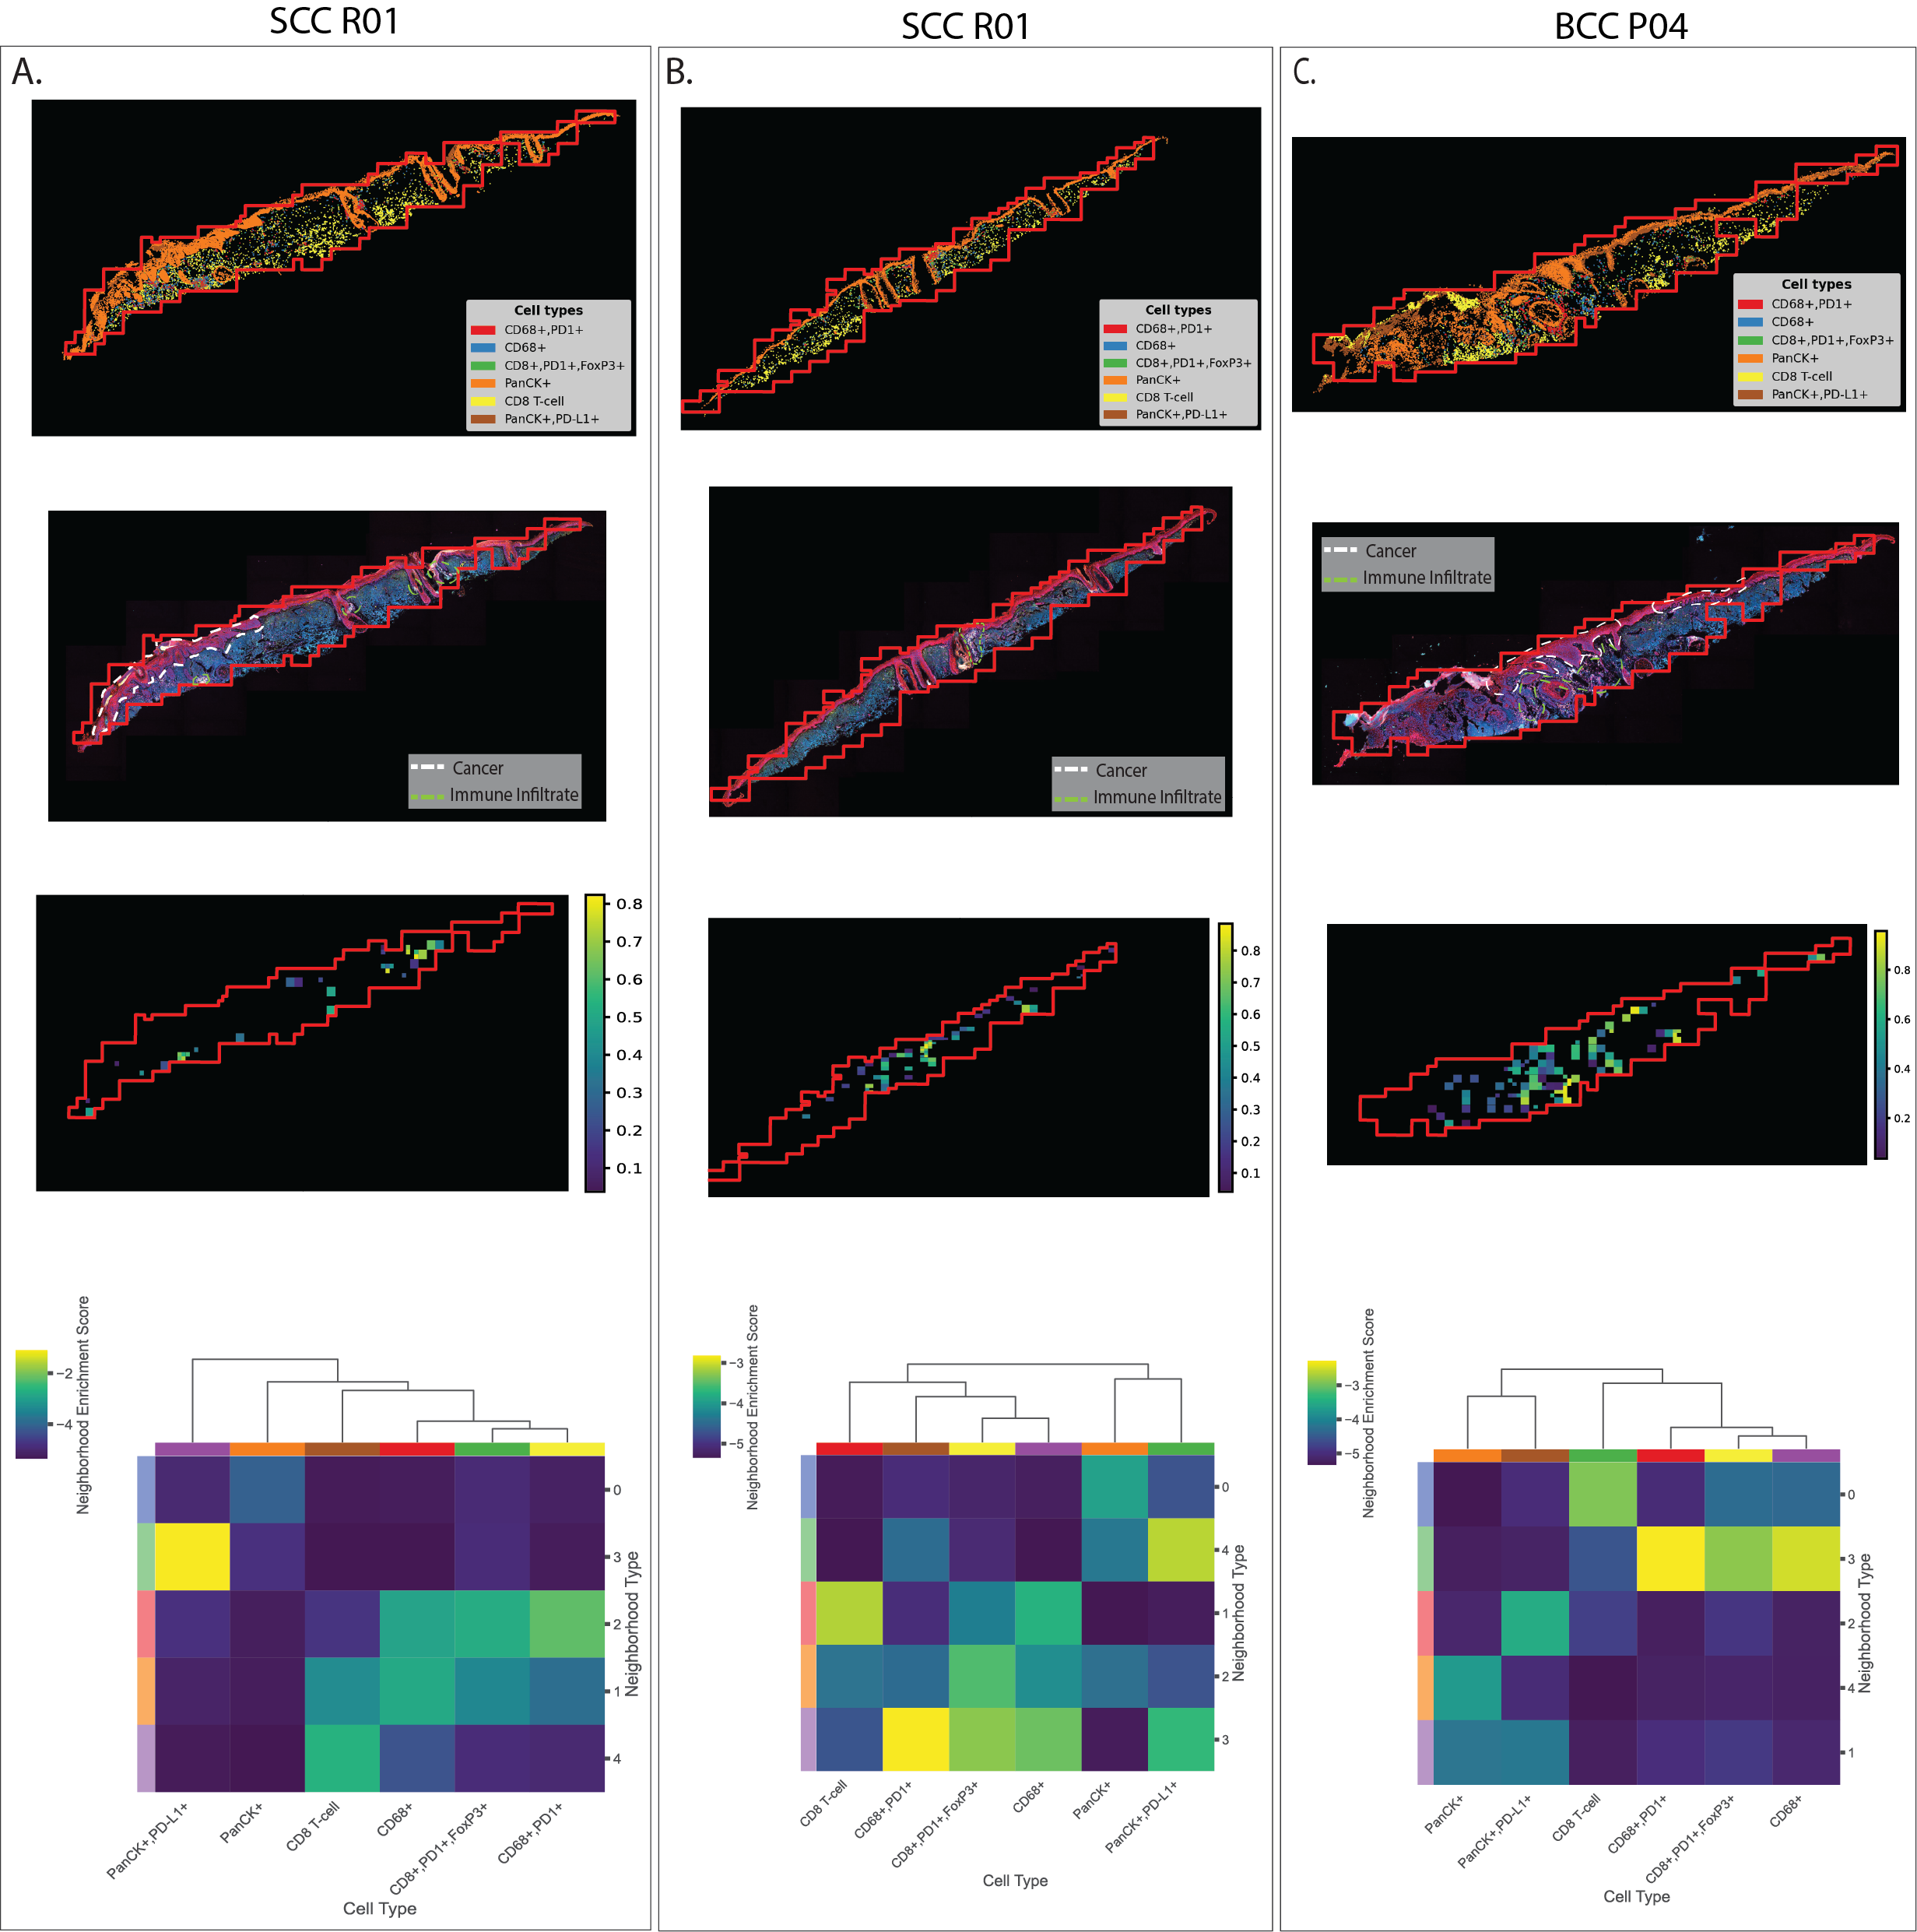
\includegraphics[width=1.0\columnwidth]{Chapter3/Figures/Chap3_supple_figure_1.png}
     \caption[Analyses results of Polaris across multiple SCC and BCC samples]{Analyses results of Polaris across multiple SCC and BCC samples. (A, B) From top to bottom are the cell type identification, pathologist annotation, the heatmap of cell colocalisation through the pair of PD1-PDL1, and the cell type composition for each cell type community detected across the tissue sample from the patient ID R01 with SCC. (C) The equivalent analysis results for the tissue samples from the patient ID P04 with BCC}
    \label{fig:Chap3_figure6}
\end{figure}
% ***************************************************


% \section{Appendix}


% \bibliographystyle{elsarticle-num}

% \bibliography{./References/Bibliography}

% There are already a few computational methods that used scRNA-seq to infer the CCC \ie CellChat \cite{jin2021CellChat}, CellPhoneDB \cite{efremova2020cellphonedb} or NicheNet \cite{browaeys2020nichenet}. However, they are all unable to address the spatial constraints of interactions. With scRNA-seq data, the limited insights into the spatial location of the RNA molecules within a cell and the organization of cells in a tissue prevent the CCC inference from reaching its potential. To address this, the development of higher multiplexed histological techniques for capturing transcriptomic or/and proteomic information at subcellular resolution, \ie co-detection by imaging (CODEX) \cite{goltsev2018CODEX} or IMC from Hyperion, facilitated the integration of spatial information into CCC inference. 

